\chapter[Linear ICS at Astra Gemini]{Linear Inverse Compton Scattering at Astra Gemini}
\label{Chap:linICS}
                                                                                                                                                                                                                                                                                                                                                                                                                                                                                    \section{Motivation}

\EliasComm{Think of more motivation that does not overlap too much with RR chapter, maybe focus more on diagnostics and specific examples. For radiation reaction studies beam parameters, ellipticity, polarisation etc. are important.}
\EliasComm{In general, measurement of intensity are also relevant.}

Linear Inverse Compton scattering (ICS) is widely used in conventional accelerators as high-energy radiation source to study nuclear processes \cite{Nakano2001_ICSNuclear} and as beam diagnostic to measure the beam energy \cite{Chouffani2006_ICS_BeamParam,Utsunomiya2014_ICS_BeamEnergy}, position \cite{Sakai2002_ICS_LaserWire}, emittance \cite{Sakai2002_ICS_EMITTANCE}, polarisation \cite{Barber1993_POL,Baylac2002_POL,Weber2018_POL} and other properties of the particle beam.

More recently it has also found application in laser wakefield accelerators as X-ray source for imaging applications, for instance of high-Z materials \cite{Banerjee2015_ICS_RADIOGRAPHY}, and since it inherits the ultrafast nature of the LWFA electron beam \cite{Lundh2011_BUNCH} it also has potential as X-ray probe for fast processes like laser-driven shocks in materials or structural transitions such as non-thermal melting \cite{Albert2016_APP}.
Linear ICS is in this context also used as beam diagnostic \cite{Jochmann2013_ICS_BeamEAngle,Golovin2016_ICS_BeamEmittance,Kramer2018_Gamma}. See for instance \cite{Corde2013_Rad,Albert2016_APP,Downer2018_DiagnosticReview} for more details and applications.

Typically, at conventional accelerators and in LWFA experiments the beam is diagnosed by scanning or rastering the laser over multiple shots through the electron beam and is focused tightly in order to produce a significant number of X-rays or gamma-rays (REF\addref). To make a meaningful measurements, this requires a stable and over many shots reproducible electron beam as available at conventional accelerator facilities or by using beam transport optics to focus the electron beam at a fixed position in space. Reproducibility and high repetition rates are already targets in the community to make laser wakefield accelerators more feasible for applications.

By increasing the intensity of the laser used as scattering beam and expanding the laser beam to a beam size larger than the electron beam, linear ICS becomes feasible as single-shot diagnostic.
In the context of radiation reaction studies, linear ICS, especially in the transient regime between linear and non-linear is useful to characterise electron beams and estimate the fluctuations.
If the gamma detector is sensitive enough this could also be used to estimate the intensity by considering the nonlinearity.

\section{Chapter Outline}

The results presented in this Chapter relate to an experimental campaign performed at the Gemini laser system in early 2019, aimed at conducting precision measurements of radiation reaction by colliding highly relativistic electron beams from laser wakefield acceleration with an intense laser pulse. Unfortunately, losing access to the scattering laser beam towards the end of the campaign due to a damaged component in the laser beam line, we were not able to perform high-intensity interactions. Nonetheless, we succeeded in colliding a relativistic electron beam with a defocused laser pulse at $a_0 \sim 0.3-0.6$ over the course of hundreds of shots, which is the data this Chapter will focus on. 

After outlining the experimental layout of the campaign, we proceed with a characterisation of the electron spectra taken at fixed experimental conditions. These are the electron spectra also to be interacted with the laser pulse to act as Compton source. 

Then results from a laser raster scan are presented: by shifting the laser beam relative to the electron beam in dual-beam shots and measuring the presence or absence of a bright gamma signal on the gamma profile detectors the size of the laser beam at the interaction plane can be established as the small and in space approximately fixed electron beam rasters the laser beam profile. This technique can be used to corroborate the spatio-temporal electron-laser alignment and estimate the change in the relative arrival time of the laser pulse and the electron beam required to achieve high-intensity interactions.

Based on the estimated laser beam parameters at the interaction and using the characterisation of the electron beams, the spectral shape of the produced radiation is discussed, followed by an estimate of the total number of high-energy photons produced in the interaction and how different spectral components of the electron beam contribute to the total yield measured on the scintillating profile screen used in the experiment.
This analysis is applied to infer the spectrum of the emitted radiation and to further constrain the conditions at the interaction. The photon yield is used to infer the beam size and intensity at the interaction point, and to diagnose the temporal fluctuations of the synchronisation of the laser pulse and the electron beam.

Based on the experimental conditions and properties of the radiation produced in this scenario, the feasibility of this light source as single-shot non-invasive electron beam diagnostic is discussed. Its applicability regarding the properties divergence, beam pointing and to resolve spatial features of the electron beam is analysed. Finally, its use to investigate the in-plasma beam dynamics of the electron bunch and the use of this diagnostic for future radiation reaction campaigns is discussed.

\section{Experimental Setup}
\label{Chap:linICS:sec:ExpSetup}

This experiment was performed at the Gemini facility in early 2019 using both laser arms of the dual laser beam facility.
A sketch of the relevant components of the setup is shown in Figure \ref{LinICS:Fig:SetupBlend}.

\subsubsection{Laser wakefield accelerator}

The driver beam for the wakefield accelerator was focused by an $f/40$ off-axis parabola (OAP) onto the leading edge of a 15 mm conical supersonic helium gas jet. The measured pulse duration was $61\pm5\,\mathrm{fs}$ \textsc{fwhm} with an average energy on-target of $12.5 \pm 0.2\,\mathrm{J}$, reaching a peak power of $195\pm3\,\mathrm{TW}$. The size of the focal spot measured $(48.6\pm3.2) \times (39.2\pm1.6)\,\mathrm{\upmu m}$ \textsc{fwhm}, amounting to a peak normalised vector potential of $a_0 = 1.88\pm0.04$ in vacuum\footnote{The focal spot data and FROG trace were analysed by Matthew Streeter (Imperial College)}. The laser was polarised in the horizontal plane.
\vspace{\baselineskip}

The exit of the gas nozzle was positioned $14\pm0.1\,\mathrm{mm}$ below the laser beam axis to avoid damage from the second, more divergent laser beam. A steel razor blade was introduced $4\pm0.1\,\mathrm{mm}$ above the nozzle edge at $- 32.4^\circ\pm 0.3^\circ$ angle in vertical direction relative to the laser axis to produce a shock front. The tip of the blade was inserted $1.2\pm0.1\,\mathrm{mm}$ into the gas flow from the same side that the driver beam enters from. 
The gas target was characterised on-shot by a transverse optical probe synchronised with the driver beam ending in a shadowgraphy and a Mach-Zehnder interferometry setup.
The interferometrically determined electron density\footnote{The interferometry data was evaluated by Cary Colgan (Imperial College)} without inserting the blade was $(1.4 \pm 0.2) \times 10^{18}\,\mathrm{cm}^{-3}$. When inserting the blade the density profile exhibits a sharp peak in density reaching about $(2.4 \pm 0.2) \times 10^{18}\,\mathrm{cm}^{-3}$, which is about twice the ambient density.
In addition to the optical probe, the gas target and the recombination light emitted by the plasma channel are imaged by a Canon DSLR camera from the side and a CCD camera from the roof of the chamber.

\begin{figure}
\centering
\includegraphics[width=0.9\columnwidth]{GeminiShock2019_ExpBlend_V1_Aug20_annotated.png}
\caption[Sketch of experimental setup to measure radiation from linear inverse Compton scattering.]{Sketch of the experimental setup aimed to measure radiation from linear inverse Compton scattering. The first laser pulse (red, left) is focused down by an $f/40$ OAP into a gas jet and accelerates electrons (blue) from LWFA, where the density perturbation induced by the blade affects the injection mechanism. A second laser is focused down by an $f/2$ OAP and counter-propagates with the electron beam performing linear inverse Compton scattering. Gamma radiation produced in the interaction (green) is emitted in the propagation direction of the electron beam and is measured downstream by a scintillating profile screen and a stack of scintillating crystals used as spectrometer (right). A converter target behind the $f/2$ OAP can be used to convert the electron beam via bremsstrahlung into an energetic calibration source for the gamma diagnostics. The electrons are dispersed horizontally by a permanent dipole magnet onto a set of Lanex screens. The accelerator, the interaction point and the magnet are in vacuum, whereas the measurement screens and gamma diagnostics are located at air separated by a thin vacuum window (orange).} 
\label{LinICS:Fig:SetupBlend}
\end{figure}
\subsubsection{Scattering beam}

A second laser pulse was focused by an $f/2$ off-axis parabola (OAP) at the opposite edge of the gas jet in a head-on geometry. The $f/2$ OAP has a 21-mm-diameter hole in the centre that allows the electrons, laser light and radiation on-axis to propagate through. A plastic ring of outer radius $28\,\mathrm{mm}$ and inner radius $11\,\mathrm{mm}$ was fitted around the hole to protect the optic and the laser chain upstream from potentially in the plasma scattered or strongly defocused laser light from the driver beam. This reduces the energy on-target by 16 percent assuming a perfect top-hat laser profile and that the collimated beam incident on the OAP has a diameter of $150\,\mathrm{mm}$. To protect the optic from potential debris a thin plastic layer with anti-reflective coating (`pellicle') and a suitable hole was attached to the mount of the OAP. The on-shot energy of the laser after the compressor was $9.73\pm 0.15\,\mathrm{J}$ and $8.17\pm0.13\,\mathrm{J}$ on-target due to the hole in the OAP. In the dataset presented, the beam diameter at the interaction was estimated to be $400\pm100\,\mathrm{\upmu m}$, which translates into $a_0 \sim 0.28 \pm 0.04$ at a pulse duration of $45\,\mathrm{fs}$. The laser was linearly polarised in the vertical plane, cross-polarised to the wakefield driver beam.

\subsubsection{Two-beam timing}

Both laser beams were synchronised to each other in vacuum to an accuracy of $\pm30\,\mathrm{fs}$ using spatial interferometry \cite{Cole2018_RR}. A 90-degree dielectric knife-edge prism (Thorlabs MRAK25-E03) was inserted at the interaction point, deflecting both beams collinearly onto the CCD chip of a camera (AVT Manta G-033B) equipped with a $\times10$ long-working-distance infinity-corrected microscope objective (Mitutoyo NIR). Due to the different radii of curvature of both beams, especially near the focus of the $f/2$ beam, a circular interference pattern emerges when the beams are overlapped in space and time. The timing procedure is explained in more detail in Section \ref{Methods:Sec:DualBeamTiming} of the \nameref{Chap:Methods}.

\subsubsection{Particle and Radiation diagnostics}

\EliasComm{If I am not using both views, should I mention this here?}

The radiation, the remaining driver laser and the electrons propagate through the hole in the $f/2$ OAP into a large aperture [$10\,\mathrm{cm} \times 30\,\mathrm{cm}$ (vertical $\times$ horizontal)] permanent dipole magnet\footnote{designed, and assembly and positioning supervised by Dominik Hollatz (Jena)} of integrated magnetic field strength $\int B(x) \mathrm{d}x = 0.35\,\mathrm{Tm}$. 
The electrons are dispersed in the horizontal plane and electrons of energy lower than 220 MeV collide with the yoke of the magnet resulting in an effective low-energy cut-off. The dispersed beam leaves the vacuum chamber through a two-layer wide-aperture vacuum window\footnote{designed and tested by the Mechanical Engineering Division at the CLF, in particular Daniel Treverrow.} of dimensions $580 \,\mathrm{mm} \,\times\, 70\,\mathrm{mm}$ (horizontal $\times$ vertical). The layer facing the vacuum consists of $25\,\mathrm{\upmu m}$ of Kapton, the outside layer is $375\,\mathrm{\upmu m}$ of Kevlar (chemical equation $C_{14} H_{14} N_2 O_4$, density $\rho = 1.44\,\mathrm{g/cm}^3$ \cite{Kevlar}) providing additional mechanical stability and fibre support that acts as mechanical fail-safe. A scintillating sensitive Lanex screen (Kodak Biomax) is placed just after the window, at $1.61\,\mathrm{m}$ distance downstream of the interaction point, to measure the spectrum of the dispersed electron beam. The screen also extends beyond the laser and radiation axis. The light and thin material of the window and the short distance to the Lanex screen minimises the impact of multiple small-angle scattering on the measurement \cite{Moller1932_Moller,Bethe1953_Moliere}.
A second Lanex screen (Kodak Standard) measures the spectrum $700\pm1\,\mathrm{mm}$ further downstream ($2.31\,\mathrm{m}$ from the interaction point) and can in conjunction with the first screen be used to account for the pointing of the beam \cite{Clayton2010_ION,Soloviev2011_TWOSCREEN}.
The screens are each imaged by a cooled 16-bit CCD camera (Andor Neo) equipped with a suitable objective and a bandpass filter transmitting light of wavelength $546\pm10\,\mathrm{nm}$. %A third camera images a small region of interest on the first screen.
\vspace{\baselineskip}

High-Z metal converter targets (bismuth, tungsten, iron) are fixed to a $1.6\,\mathrm{mm}$ plastic (PTFE) base and mounted on a motorised linear stage between the mount of the $f/2$ OAP and the dipole magnet. The targets can be driven into the beam path to intercept the electron beam and to produce gamma radiation from bremsstrahlung \cite{Glinec2005_Brems} to calibrate the gamma-ray diagnostics in this experiment \cite{Behm2018_Gamma}. The high-Z targets enable efficient conversion of the electron beam energy into radiation, but do not allow measuring the electron spectrum at the same time. The PTFE base itself can also be used as converter that is less efficient in terms of radiation yield but allows a synchronous measurement of the electron and gamma-ray beam. 

Radiation traverses the magnet on the laser axis, then passes through a $120\,\mathrm{\upmu m}$ aluminium laser beam block terminating the wakefield driver beam, and the Kevlar-Kapton window mentioned before. Bright radiation in the right bandwidth is also captured by the Lanex screen as it extends beyond the laser and radiation axis. An array of $45 \times 45$ scintillating with thallium doped caesium-iodide (CsI:Tl) crystals of dimensions $1\,\mathrm{mm} \times 1\,\mathrm{mm} \times 10 \,\mathrm{mm}$ measures the profile of the radiation $700 \pm 1\,\mathrm{mm}$ downstream from the plane of the first Lanex screen. The crystals are each separated transversely by a $0.2\,\mathrm{mm}$ thick $TiO_2$ coating and are held together by a $TiO_2$ front plate of thickness $0.5\mm$. The stack covers a field of view corresponding to a cone of half opening angle $11.7\,\mathrm{mrad}$. The spatial resolution including the coating separating the individual crystals is then $1.2\,\mathrm{mm}/2.31\,\mathrm{m} = 0.52\,\mathrm{mrad}$.
$704 \pm 1\,\mathrm{mm}$ further downstream from the profile screen another elongated array of caesium-iodide crystals is positioned to measure the spectrum of the gamma radiation. Both scintillator arrays, the profile screen and the spectrometer, are imaged using cooled 14-bit EMCCD cameras (Andor iXons). The diagnostics are described in more detail in Section \ref{Methods:Sec:GammaDiags} of the \nameref{Chap:Methods}.

\section{Characterisation of Electron Spectra}
\label{Chap:linICS:sec:Espec}


\begin{figure}
\centering
\includegraphics[trim={4.0cm 0 3cm 0}, clip, width=1.0\columnwidth]{Example_Montage_twoSets_V2.png}
\caption[Waterfall plot for electron spectra at fixed conditions.]{Waterfall plot of electron spectra measured at fixed experimental conditions. The y-axis indicates the electron energy in MeV, the x-axis shows the order the shots were taken in. The electron spectra measured on the Lanex screens were integrated in the non-dispersion axis and each occupy one column in this waterfall plot. The colour scale indicates the charge per MeV in the beam.}
\label{linICS:Figs:fixed_waterfall}
\end{figure}

In this experiment the electrons were injected through density perturbations in the supersonic gas flow which were introduced by a steel blade \cite{Schmid2010_SHOCK} and subsequently accelerated to relativistic energies via laser wakefield acceleration (LWFA). The electron spectrum was measured by scintillating Lanex screens as part of a magnetic spectrometer setup. The image processing of the data is not further elaborated here but can be found for instance in \cite{ColeThesis,PoderThesis} or Section \ref{Chap:Methods:Sec:Espec} of the \nameref{Chap:Methods}. We will only consider the measurements from the first Lanex screen and ignore errors in the inferred electron energy due to global pointing fluctuations \cite{Clayton2010_ION,Soloviev2011_TWOSCREEN}.

We consider a dataset consisting of a series of shots at fixed conditions to investigate fluctuations in the accelerator performance. These electron beams were collided with the laser pulse and will in the following analysed in more detail for radiation production through inverse Compton scattering.
The dataset consists of 386 shots with electron beams, taken at constant backing pressure of the gas jet and fixed blade position ($1.2\pm0.1\,\mathrm{mm}$ into the gas flow from the entry point of the driver beam). A waterfall plot of the in non-dispersion direction integrated electron spectra is shown in Figure \ref{linICS:Figs:fixed_waterfall}. Despite the constant conditions, the properties of the electron beams vary strongly from shot-to-shot and beams of a wide range of shapes, maximum energy and energy spread are measured. A few examples of the 2D electron spectra from the dataset are provided in Figure \ref{linICS:Figs:Elec_example}.
The spectral bandwidth of the beams varies strongly with some exhibiting an almost flat spectrum spanning hundreds of MeV (see 4 left panels in Figure \ref{linICS:Figs:Elec_example}). These spectrally very wide electron beams show signatures of strong transverse oscillations which indicate their potential to act as a bright betatron source \cite{Corde2013_Rad}. In other instances electron beams with narrow energy spread around $1\,\mathrm{GeV}$ are measured (right panels in Figure \ref{linICS:Figs:Elec_example}). 
\SMComm{Can you sort this not in shot number but laser energy or charge to see whether there is any systematics?}

\begin{figure}
\centering
\includegraphics[trim={4cm 0 1cm 0}, clip, width=1.0\columnwidth]{Example_Espec_CollisionMontage_V3.png}
\caption[Examples of 2D electron spectra measured in the experiment.]{Examples of 2D electron spectra measured in the experiment. The y-axis is the dispersion axis and shows the electron energy in MeV on a linear scale, the x-axis indicates the divergence in mrad. The colour scale indicates the amount of charge per MeV per mrad in the beams and is fixed for all plots. Projections of the beams are shown on the respective axes: on the x-axis the over the dispersion-axis integrated spectrum is shown and is equivalent to the horizontally integrated spatial profile of the beam and is shown as charge per mrad as a function of divergence in mrad. The projection on the y-axis is the in non-dispersion axis integrated spectrum as also shown in the waterfall plot in Figure \ref{linICS:Figs:fixed_waterfall} and shows the charge per MeV as a function of the electron energy in MeV. The amplitude of the projections is fixed across all panels and is not representative of the relative charge between the panels.}
\label{linICS:Figs:Elec_example}
\end{figure}

The striking variability of the electrons produced in this dataset at seemingly fixed experiment conditions is not consistent with experimental results reported from other LWFA experiments at other laser systems using shock injection \cite{Schmid2010_SHOCK}. These setups typically provide reproducible electron beams with narrow energy spread \cite{Schmid2010_SHOCK,Buck2013_SHOCK,Swanson2017_SHOCK,Tsai2018_SHOCK}. 
\vspace{\baselineskip}

\begin{figure}
\centering
\includegraphics[trim={6cm 0 6cm 0}, clip, width=1.0\columnwidth]{linICS_ElectronProperties_Histograms_V2.png}
\caption[Histogram of fluctuations in the electron beam properties in this dataset.]{Histograms showing the fluctuations of electron properties in course of this dataset (386 shots). Top left: Total charge of the electron beams measured from 220 MeV upwards. Top right: Maximum electron energy, defined as energy at which the spectral intensity falls to 10 percent of its peak value. Bottom left: \textsc{fwhm} Vertical divergence (non-dispersion axis) in mrad. Bottom right: Beam pointing fluctuation in mrad from the mean position. }
\label{linICS:Figs:Elec_histogram}
\end{figure}

The key properties of the electron beams in this dataset are summarised in Figure \ref{linICS:Figs:Elec_histogram} in form of histograms showing charge, maximum electron energy, vertical (non-dispersion axis) divergence and beam pointing.
The maximum energy of the electron beam, here defined as the energy when the spectral intensity reaches 10 percent of its peak value, measured on average $944\pm139\,\mathrm{MeV}$, with some shots reaching up to $1.3\,\mathrm{GeV}$. The charge of the beam varied in particular due to the varying spectral range of the bunch with a mean of $239 \pm 92\,\mathrm{pC}$.
The divergence of the beams was measured to be $2.7\pm 2.5\,\mathrm{mrad}$ and the vertical position of the beam centroid was fluctuating by $2.2\,\mathrm{mrad}$. The indicated errors are the standard deviations from the on average measured value, i.e. the statistical error and not a measurement error.
\SMComm{Use median, upper, lower quantiles etc. equivalent to standard deviation but here not normal. Overestimating error and implying sub-zero divergence.}
\vspace{\baselineskip}

The wide range of electron beams produced in this setup is interesting in the context of radiation production by linear inverse Compton scattering (ICS). Since the properties of the beams this accelerator generates vary strongly, the radiation these electron beams are capable to produce in a well-defined linear ICS interaction will also vary significantly. This means that this accelerator is in principle also able to produce a wide range of radiation spectra from broadband to strongly peaked radiation, but an increased control over the accelerator would be required to shape the spectral emission and develop a tunable radiation source that can be optimised for a respective application. 
\SMComm{Check any correlation with laser energy or similar. Maybe add to histograms.}

\section{Laser raster scan}
\label{Chap:linICS:Sec:RasterScan}
\begin{figure}[h]
\centering
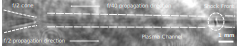
\includegraphics[width=0.8\columnwidth]{RasterScan_Shadowgraphy_CloseUp_annotated.pdf}
\caption[Shadowgram of the plasma channel with the focusing f/2 laser cone.]{Cut-out of a shadowgram of the gas jet taken with the transverse optical probe (horizontal plane). The wakefield driver beam enters the gas jet from the right side and generates a plasma channel. The dark line on the right side results from a shock front. The second scattering beam is focused tightly into the plasma from the left side, where a converging cone becomes visible. The spatial scale is indicated in the bottom right corner.}
\label{linICS:Figs:ShadowgraphyRaster}
\end{figure}


The two laser beams were overlapped in space and time in vacuum using a photodiode and spatial interferometry (see Section XX in the \nameref{Chap:Methods}). On full-power shots the cone of the scattering beam focusing into the plasma is visible on the transverse (horizontal plane) shadowgraphy diagnostic (see Figure \ref{linICS:Figs:ShadowgraphyRaster}, left side) along with the plasma channel from the wakefield driver beam and the shock leading to the injection of electrons into the wakefield accelerator (dark line in the plasma channel on the right side).

On full-power shots with both laser beams and an electron beam produced in the wakefield accelerator, we consistently measured a bright circular or oval signal on the gamma profile screen indicating an interaction of the laser pulse and the electron beam (linear inverse Compton scattering). The consistency of the collisions indicates that the laser beam is larger than the electron beam and the combined fluctuations in the relative position of the scattering beam and the electron beam.
To establish the transverse size of the scattering laser pulse at the interaction point, the scattering laser beam was shifted in one transverse axis by translating the position of the $f/2$ OAP, assuming that the laser beam translates by the same amount for small motions. The remaining experimental parameters and the alignment of the wakefield driver beam were kept constant during this procedure. At each OAP position at least 5 full-power dual-beam shots were taken. If at least one of the lasers was not firing or no electron beam was measured on-shot additional shots were taken in order to accumulate 5 suitable data points at each OAP position. The response of the gamma profile screen was recorded and the number of visible bright signals was noted down. The OAP was then translated by $50\,\mathrm{\upmu m}$ and the procedure was repeated. In Figure \ref{linICS:Figs:GammaProfileRaster} a montage of the gamma profile screens at each position of a horizontal scan in the OAP position is shown. The relative position from the established beam centre is shown on the x-axis. The integrated gamma yield on the profile screen measurements is shown in Figure \ref{linICS:Figs:GammaProfileRasterCounts}. When there were no bright signals observed on the gamma profile screen for two consecutive OAP positions, this was deemed to be a suitable indication of no overlap of the laser beam and the electron bunch. The distance mapped by this method includes the diameter of the laser beam at the plane of the interaction at that transverse position and the fluctuations in the relative beam pointing of laser and electron beam, and the size of the electron beam. Since the finite step size in the OAP translation ($50\microns$) is much larger than the expected electron beam size and the relative pointing fluctuations, the dominant error on the transverse size of the laser beam is the step size.

\begin{figure}
\centering
\includegraphics[trim={8cm 2.5cm 6cm 2.5cm}, clip, width=1.0\columnwidth]{linICS_RasterScan_GammaProfile_Montage_V3.png}
\caption[Montage of gamma profile measurements taken during an OAP raster scan.]{Montage of gamma profile measurements at different transverse OAP positions. Each panel shows a the measured gamma profile images for a series of shots taken at a fixed OAP position. The panels are labelled with the relative transverse offset of the OAP for that particular dataset. The colour scale indicates the measured yield of scintillation light which is proportional to the energy deposited in the profile stack, but is not constant across the panels.}
\label{linICS:Figs:GammaProfileRaster}
\end{figure}

If we assume that this method successfully determines the transverse extent of the scattering beam at the plane of the interaction, we can also pinpoint the centre of the laser pulse by shifting the OAP to the central position between the outermost OAP positions on which a significant gamma signal was measured on-shot. By repeating this procedure in the second transverse dimension we can accurately centre the scattering laser pulse on the electron beam in both transverse dimensions, provided that the relative pointing fluctuations and the electron beam size are negligible. The accuracy of this procedure can be improved by repeating the steps in the first transverse dimension in a third pass and by reducing the step size of the OAP translation. The principle of this `raster scan' resembles the `laser wire' or spatial cross-correlation technique where a scattering laser beam is focused tightly onto an electron beam to produce energetic from linear inverse Compton scattering and to diagnose the electron beam \cite{Alley1996_LaserWire,Leemans1996_ICS_BeamTransLong,Okugi1999_WireScanner_Emittance,Sakai2001_BeamSize,Sakai2002_ICS_LaserWire,Honda2005_ICS_LaserWire,Chen2013_ICS,Jochmann2013_ICS_BeamEAngle,Golovin2016_ICS_BeamEmittance,Kramer2018_Gamma}. The laser focus is typically smaller than the electron beam at the plane of the interaction and the transverse size of the electron beam can be determined by translating the laser focus transversely over multiple shots. The emission spectrum and angular distribution of the backscattered radiation can also be used as diagnostic for other beam properties. The name `laser wire' is derived from the physical wire scanners that were used as beam diagnostics in conventional accelerator facilities \cite{Okugi1999_WireScanner_Emittance}. In the case presented here, the electron beam, however, is much smaller than the laser beam. Even though the laser pulse is translated as in a laser wire whilst the electron axis remains fixed, here the electron beam effectively acts as the probe and diagnoses the laser beam at the interaction plane, inversely to the laser wire.

\EliasComm{Matt mentioned he thought about using a Bayesian inference model on this and automate this process. This is actually a great idea and would make it possible to get to high-intensity interactions and take loads of data. \cite{Streeter2018_TEMPFEEDBACK,Streeter2019_RASTERSCAN}}

\subsubsection{Experimental Results}

\begin{figure}
\centering
\includegraphics[trim={4cm 0cm 4cm 0cm}, clip, width=1.0\columnwidth]{linICS_RasterScan_GammaProfile_Counts.png}
\caption{Integrated pixel counts on the gamma profile screen for different OAP positions.}
\label{linICS:Figs:GammaProfileRasterCounts}
\end{figure}

In the raster scan presented in Figure \ref{linICS:Figs:GammaProfileRaster} and Figure \ref{linICS:Figs:GammaProfileRasterCounts} the interaction region and hence, following our argument, the combined size of the laser beam and the electron beam along with variations in the relative beam pointing is $400\pm100 \,\mathrm{\upmu m}$. The integrated gamma yield in Figure \ref{linICS:Figs:GammaProfileRasterCounts} also shows signs of a drop in intensity throughout the scan, potentially when crossing the hole in the beam. At an energy on-target of $9.73\pm0.15\,\mathrm{J}$ this amounts to an average $a_0 \approx 0.28 \pm 0.04$, where we assumed a perfect flat-top beam profile and hence ignored the reduction of the energy in the beam due to the hole in the $f/2$ OAP as this does not affect the photon density in the near-field. For an $f/2$ geometry this also indicates that the interaction occured at $\sim1.1\pm0.1\,\mathrm{mm}$ distance from the focal plane. Based on the alignment procedure in the experiment we suspect that the interaction occurs prior to the focus of the scattering beam (left hand side in Figure \ref{linICS:Figs:ShadowgraphyRaster}). In either case the interaction occurs in the plasma, so that the electron beam is only $\sim \mathrm{\upmu m}$ in size \cite{Weingartner2012_BUNCH} and spatial fluctuations due to pointing variations of the laser with a varying off-axis distribution due to betatron oscillations with betatron amplitudes of typically $r_\beta \sim \mathrm{\upmu m}$ \cite{Corde2013_Rad}. Since the beam pointing of the $f/2$ beam is demagnified due to the short focal distance, the raster scan mainly reflects the dimensions of the scattering beam and this is hence a suitable method to determine the size of the laser beam.
\SMComm{Find a better metric. number of successful shots, Qgamma relation or similar. This could then also be used for Matt's Bayesian.}
\SMComm{Ask Matt about proper Bayesian paper.}
\SMComm{Replot with other scaling as second?}

The gas jet expands from its nozzle opening diameter of $15$ mm to a length of approximately $17.3$ mm (measured by the length of the plasma channel on the shadowgram). This means based on this scan the interaction point is defined as intended by the alignment procedure, the inner edge of the gas nozzle, but the gas jet has expanded. In addition, the focal plane of the laser has changed. We have to keep in mind that translating the OAP in longitudinal direction does not change the intensity of the interaction at first order as we shift the interaction plane along with the intensity plane when doing so. If we want to change the intensity at the interaction we have to change the relative delay of the two laser pulses.
In brief, shifting the longitudinal OAP position and the focal plane in space only changes the plane of interaction at roughly the same intensity, whereas shifting the delay of the beams shifts both the interaction plane and the intensity. The mismatch of the interaction plane and the focal plane might be due to a misunderstanding of these two mechanisms and we mistakenly `compensated' for the shift in focus and fixed the interaction plane, rather than the intensity at the interaction.
\SMComm{Confirm with Matt and Brendan whether this makes sense and matches their memory.}

\begin{figure}
\centering
\includegraphics[trim={4.5cm 0 5cm 0}, clip, width=.9\columnwidth]{linICS_Raster_WaistSize_V2.png}
\caption[Waist size of a Gaussian laser beam focusing with an $f/2$ optic as a function of distance from the focal plane.]{Waist size of a Gaussian laser beam focusing with an $f/2$ optic as a function of distance from the focal plane. By establishing the size of the laser beam with a raster scan one can then adjust the relative arrival time of the electron beam and the laser pulse to move the interaction plane into the high-intensity focus. If one moves the delay in the wrong direction, one will then see a larger beam at lower intensity which can be confirmed by another raster scan before then moving to the right relative timing for high-intensity collisions.}
\label{linICS:Figs:RasterTemporalTranslationIdea}
\end{figure}
\EliasComm{Add some features to Figure 4.8.}

\subsubsection{Laser raster scan as tool to achieving high-intensity interactions}

By determining the centre of the beam and its transverse size at the interaction, i.e. using a spatial correlation technique, the position of the plane at the interaction relative to the focal plane and their relative alignment in the transverse direction can be determined. The spatial offset between the plane of the interaction and the focus of the laser pulse can be compensated by adjusting the beam path of either laser pulse. At Gemini beam path can be removed or added at micrometre precision by a motorised delay stage in the laser area on the `split-and-delay' (SAD) table.
After adjusting the relative timing the beam size can be confirmed by repeating the raster scan at the new interaction plane. This procedure is visualised in Figure \ref{linICS:Figs:RasterTemporalTranslationIdea}. Interactions near the focus will be signalled by particularly bright gamma-ray yield but also by less consistency in the interactions as the size of the pointing fluctuations become comparable to the beam size. If aligning the laser pulse and the electron beam using this method requires a significant shift of the OAP in transverse direction, it might also become necessary to re-optimise the OAP angle as a translation of the optics might have introduced an astigmatism into the beam.

Unfortunately, in the experiment the final step of shifting the interaction plane to the high-intensity focus of the scattering laser pulse was not possible. A lens in the beam expander telescope of the scattering beam broke during this dataset and we were not able to continue the campaign with dual-beam shots and potential high-intensity collisions.
Nonetheless, we were able to show consistent overlap in space and time and a good control over the spatio-temporal alignment. The laser raster scan promises to become a useful technique to estimate the laser intensity at the interaction plane and to systematically achieve high-intensity collisions in a future measurement of radiation reaction.

\section{Gamma spectra from inverse Compton scattering}


A photon of energy $E_{ph}$ that is scattered from a relativistic electron is Doppler up-shifted due to the relativistic Lorentz boost. The energy of a scattered photon, $E_{X}$, is given by \cite{Esarey1993_NT}:
\begin{equation}
E_{X} = E_{ph}\times\frac{2(1-\cos \theta)\gamma^2}{1+a^2_0/2 + \gamma^2 \theta^2_0},
\label{linICS:eqns:full_linICS}
\end{equation}
where $\theta$ the angle between the electron and the incoming photon, $a_0$ is the normalised vector potential and $\theta_0$ is the angle of the observer relative to the propagation direction of the electron.

The electron beams shown in Section \ref{Chap:linICS:sec:Espec} were collided with a laser pulse at an intensity of $a_0 < 0.3$, as estimated in the previous section (Section \ref{Chap:linICS:Sec:RasterScan}). This is below $a_0 = 1$ such that at first order we can ignore the contribution of higher harmonic radiation and only consider the fundamental harmonic from linear inverse Compton scattering \cite{Esarey1993_NT}. Since then also $a^2_0 \ll 1$ we can also ignore the term $a^2_0/2$ in the denominator, which accounts for red-shifting of the radiation when the longitudinal component of the electron motion becomes significant (see Chapter \ref{Chap:Theory:SingleParticle} for `figure-of-eight motion') (REF\addref). 

The electron beams are in most cases confined to a divergence cone of few milliradians (REF\addref). For a beam of divergence $4\,\mathrm{mrad}$ the difference introduced by the electron angles in the $\cos\theta$ term, assuming a collimated light source is less than $0.001\%$, which means that we can ignore a broadening of the spectrum from electron angles as well.

For a beam focused by an $f/2$ optic the angle between the outer rays is up to 14.04 degrees which corresponds to a 3 percent spread in energy. Since the electron beam $w_0 \sim \microns$ only interacts with a small fraction of the full beam with radius $r$, i.e. $\pi w^2_0/\pi r^2 \ll 1$, the rays in the interaction region are approximately collinear and this contribution can be ignored as well. A global shift of the radiation by 3 percent due to the relative pointing of the electron beam and the laser pulse within the solid angle is also negligible for our considerations ($\Delta E <1\MeV$ at $30\MeV$).

\begin{figure}
\centering
\includegraphics[trim={4cm 0 4cm 0}, clip, width=.6\columnwidth]{Egamma_ICS_V2.png}
\caption[Gamma energy produced in scattering a 1.55 eV photon with a relativistic electron beam in a head-on collision.]{Gamma energy in MeV produced in scattering a 1.55 eV photon with a relativistic electron beam in a head-on collision as a function of electron energy in MeV. The relation is calculated with the simple Equation \eqref{linICS:Eqs:SimpleLinICSEX}, which ignores energy broadening or reduction due to relative angles of electron beam and laser pulse, redshifting or off-axis emission.}
\label{linICS:fig:ElecEToEgamma}
\end{figure}

In linear ICS scattered photons in a head-on collision will be emitted in a narrow cone of divergence $\sim 1/\gamma \ll 1$ \cite{Corde2013_Rad}, such that we will only measure and consider on-axis emissions, $\theta_0 \approx 0$.
For $\gamma \sim 2500$ ($\epsilon \sim 1.3\,\mathrm{GeV}$) and $a_0 = 0.3$
\begin{equation}
\psi = \gamma^2 a_0 \frac{2 r_e \omega}{3c} \ll 1,
\end{equation}
which indicates that radiation reaction effects are negligible and the interaction with the laser pulse does not perturb the electron beam significantly as a whole \cite{Thomas2012_LL,Albert2016_APP}.
Combining these assumptions and considering a head-on collision ($\theta = 180^\circ$) Equation \eqref{linICS:eqns:full_linICS} above simplifies to
\begin{equation}
\boxed{E_X \approx 4\gamma^2 E_{ph}.}
\label{linICS:Eqs:SimpleLinICSEX}
\end{equation}

For a titanium-sapphire laser system with central wavelength $800\,\mathrm{nm}$ like Gemini the corresponding energy carried by an individual photon, $E_{ph}$, amounts to $1.55\,\mathrm{eV}$. Based on the simplified Equation \eqref{linICS:Eqs:SimpleLinICSEX} above and ignoring the bandwidth of the laser, we then obtain a quadratic one-to-one mapping of the electron energy to a corresponding gamma-ray energy (see Figure \ref{linICS:fig:ElecEToEgamma}). 
\vspace{\baselineskip}

\begin{figure}
\centering
\includegraphics[trim={1cm 0 1cm 0}, clip, width=1.0\columnwidth]{Example_Espec_ICS_V3.png}
\caption[Example of two electron spectra with corresponding calculated ICS spectrum.]{Example of two in non-dispersion axis integrated electron spectra from the dataset presented earlier. The y-axis indicates the charge per MeV in the spectrum and the x-axis the electron energy in MeV. The spectra are normalised to their peak value of charge per MeV. The to the electron energies corresponding gamma-ray energies as calculated using Equation \eqref{linICS:Eqs:SimpleLinICSEX} are indicated in a second non-linear x-axis on the top.}
\label{linICS:fig:ElecEToEgamma_Examples}
\end{figure}

Since the properties of the electron beam measured in this experiment vary strongly, we also expect the spectrum of the radiation produced from linear ICS to follow this behaviour. In this scenario the cross section is independent of the electron energy \cite{Albert2016_APP} and the spectral shape of the electron beam is preserved in the gamma spectrum. Two examples of electron spectra and the with Equation \ref{linICS:Eqs:SimpleLinICSEX} calculated corresponding gamma-ray spectra are shown in Figure \ref{linICS:fig:ElecEToEgamma_Examples}. One electron beam is spectrally very broad (red) with significant spectral intensity spread from below the measurement threshold of $220\,\mathrm{MeV}$ up to $1200\,\mathrm{MeV}$, resulting in a gamma-ray spectrum from few to $35\,\mathrm{MeV}$. The other beam (blue) is strongly peaked at just under $1.2\,\mathrm{GeV}$ with narrow energy spread of $< 10\%$, which has the potential to be converted into a narrow energy spread gamma-ray source centred at $34\,\mathrm{MeV}$.

\section{Number of scattered photons}

Based on the conditions in the experiment and the inferred intensity at the interaction (see Section \ref{Chap:linICS:Sec:RasterScan}), we assume that the interaction is correctly described by linear ICS.
The number of photons scattered or the number of produced gamma-rays, $N_X$, in the interaction of the laser pulse with an electron beam of size $w_0$ is approximated by \cite{Albert2016_APP}
\begin{equation}
\boxed{N_X = \frac{\sigma_T}{\pi w^2_0} N_L N_e,}
\end{equation}
where $\sigma_T = 6.65 \times 10^{-25}\,\mathrm{m}^{-2}$ is the Thomson scattering cross-section, $N_e$ the number of electrons involved, $N_L$ the number of laser photons and $w_0$ the waist size. In this limit the cross-section and the total number of photons produced is independent of the electron and photon energy.

The Rayleigh length, $z_R$, of an $f/2$ beam is approximately $2.5 \lambda f^2_\# \approx 8\,\mathrm{\upmu m}$.
At a diameter of $400\pm100\,\mathrm{\upmu m}$ the beam is at $\sim 1100\pm 275 \mathrm{\upmu m}$ distance from the focal plane, which corresponds to $> 100 z_R$, so that the laser is in its near field at this plane. As discussed before we ignore relative angles between the laser and the electron beam. We will also ignore focusing effect assuming that the duration of the interaction is short enough due to the short length of the laser pulse and the electron bunch \cite{Lundh2011_BUNCH} to avoid significant changes in intensity such that the electrons encounter a static photon field. Since the laser beam is much larger than the electron beam, we assume that the entire electron beam passes through the laser pulse and that all electrons encounter the same photon density, hence also contribute equally to the total radiation produced as the cross-section is constant across the energies.
Assuming a homogeneous perfect flat-top laser profile we estimate the number of photons interacting with an electron beam of transverse area $\pi w^2_0$ as the on-shot energy measurement (without the hole), $E_J$, divided by the energy of a single photon, $E_{ph}$, times the ratio of the area of the laser beam that overlaps with the electron beam and the full laser beam area at the plane of the interaction:

\begin{equation}
N_{ph} = \left[\frac{E_J}{E_{ph}} \frac{\pi w^2_0}{\pi r^2}\right].
\end{equation}

We then obtain for the number of scattered photons, $N_X$:
\begin{align}
N_X &= \frac{\sigma_T}{\pi w^2_0} \left[\frac{E_J}{E_{ph}} \frac{\pi w^2_0}{\pi r^2}\right] \left[\frac{Q}{e}\right],\\ \nonumber
&= \frac{\sigma_T}{\pi r^2}\left[ \frac{E}{E_{ph}}\right] \left[ \frac{Q}{e}\right],
\end{align}
where $E_J$ is the energy in the laser pulse, $E_{ph}$ the energy of a single photon and $r$ the radius of the beam at the plane of the interaction. The region of the interaction defined by the electron beam size $w_0$ cancels out as the photon density is constant across any region in this approximation.
In useful units we can write
\begin{equation}
\boxed{N_X = 5.32 \times 10^{10}\times  E [J] \times Q [100pC] \times r[\mu m]^{-2}.}
\label{Chap:linICS:Eqn:NX_UsefulUnits}
\end{equation}
Using the conditions in the experiment in this equation ($E_J = 9.73\pm0.15$,$Q=239\pm92\,\mathrm{pC}$ and $r=200\,\mathrm{\upmu m}$) we estimate that $(3.1 \pm 1.2) \times 10^{7}$ photons are on average scattered and emitted at an energy $E_X > 1\,\mathrm{MeV}$. This is of similar order of magnitude as reported for similar Compton experiments and bright betatron sources \cite{Kneip2010_BETATRON,Chen2013_BETATRON}, where we can assume that the radiation has a to the electron beam comparable pulse duration and source size (REF\addref).
\EliasComm{Maybe add a contour plot to show how the downscaling works.}
\vspace{\baselineskip}

However, considering the experimental parameters it becomes clear that a linear Compton source can be achieved in a much more economical way by scaling down the energy and the beam size at the interaction, whilst still preserving a permanent overlap within the shot-to-shot fluctuations of the laser and the accelerator. Assuming a fixed charge in the electron beam, the number of scattered photons then only depends on the ratio of the laser energy and the beam size $\sim E/r^2$. By reducing the beam radius from $200\,\mathrm{\upmu m}$ to $25\,\mathrm{\upmu m}$, a factor of 8, the corresponding energy in the scattering beam can be reduced by a factor of 64, to about $150\,\mathrm{mJ}$, to produce the same number of photons as before. Using an $f/2$ OAP as in this case, the plane of the interaction would be more than 10 Rayleigh lengths, $z_R$, away from the focal plane and which might still be in the near-field of the laser, where the profile is flat and smooth, such that any change in response would predominantly reflect the electron beam properties.

\section{Energy-dependent detector response}

\begin{figure}[h]
\centering
\includegraphics[trim={4.8cm 0 5cm 0}, clip, width=0.8\columnwidth]{Edep_Jena_1_100_MeV.png}
\caption[Energy deposition in gamma profile detector as function of photon energy as simulated in GEANT.]{Energy deposition per photon in the gamma profile stack as a function of the incident photon energy in MeV as simulated in GEANT4.}
\label{linICS:Figs:Edep_ResponseGEANT}
\end{figure}

In the previous sections we calculated how an electron spectrum translates with linear ICS into a gamma spectrum, and estimated the number of high-energy photons produced in such an interaction, finding that the cross-section in this regime is independent of the electron or gamma-ray energy, respectively.

However, whilst the cross-section for an interaction is independent of energy and, as a result, also the number of emitted photons per electron and energy band, the contribution to the detected yield on the gamma profile detector will not necessarily be constant across different energies. The gamma profile detector is not a calorimeter and only absorbs a fraction of the total radiation passing through it. Since there is a range of mechanisms coming into play at the tens of MeV photon energy range, the energy deposition in the profile screen was simulated using GEANT4 \cite{GEANT4} for a range of photon energies. The simulated average energy deposited by one individual photon incident the profile stack is shown in Figure \ref{linICS:Figs:Edep_ResponseGEANT} as a function of the photon energy, $E_\gamma$. Between $E_\gamma=1$ and $15\MeV$ the energy deposition increases steadily before slowing down and increasing at a slower rate over the remaining energy range. This is important when we want to estimate the total number of photons from a measurement in the experiment, as we have to assume a spectral shape and scale it accordingly. The energy-dependency shown in Figure \ref{linICS:Figs:Edep_ResponseGEANT} contrasts the almost flat energy deposition of relativistic electron beams in Lanex as discussed in \cite{Glinec2006_Lanex}.

\begin{figure}
\centering
\includegraphics[trim={1cm 0 1cm 0}, clip, width=1.0\columnwidth]{Example_Espec_ICS_Edep_V3.png}
\caption[Energy-dependent contribution to yield on detector for a given electron spectrum.]{Example electron spectrum and weighted contribution to the total yield as measured on the gamma profile screen. The y-axis shows the charge per MeV as function of the electron energy (x-axis). The x-axis on the top indicates the corresponding gamma-ray energy via linear ICS. The blue curve shows the spectrum as before. In the red curve the y-value is weighted by the energy deposited per photon and hence shows how much energy is being deposited. Both curves have been normalised such that the peak value at 1200 MeV takes the value 1.}
\label{linICS:Figs:Edep_Response}
\end{figure}
In Figure \ref{linICS:Figs:Edep_Response} an example electron spectrum is given, its related gamma spectrum and the relative contributions in terms of total energy deposition. The response of a detector would in this case be dominated by the high energy peak and the radiation from lower energy electrons is in relative terms suppressed. The response of a profile screen as we use it in this experiment then mainly reflects the properties of the higher tail of the radiation. If one is mainly interested in the properties of the high-energy electrons this is of advantage, as one would be in radiation reaction studies.
\vspace{\baselineskip}

Using the simulated result as a lookup-table for the energy deposition and relating the photon energy to the electron energy, the total energy deposition, $\mathcal{E}_{dep}$, for a given electron spectrum can be calculated as follows:
\begin{equation}
\boxed{\mathcal{E}_{dep} = \int E_{dep} (\gamma) \frac{\sigma_T}{\pi \omega^2_0} N_L \frac{\mathrm{d}N_e}{\mathrm{d}\gamma}\mathrm{d}\gamma  \approx \langle E_{dep} (\gamma) \rangle N_X.}
\label{linICS:Eqs:Edep_YIELD}
\end{equation}
This becomes in particular important when the electron spectrum covers a wide energy range as in some of the cases presented. Higher energy radiation contributes in relative terms more to the response of the measured profile.

\begin{figure}
\centering
\includegraphics[trim={4cm 0 4cm 0}, clip, width=1\columnwidth]{linICS_FULL_NxNxEXP_Plot_V2.png}
\caption[Estimated number of scattered photons]{Estimated number of scattered photons based on the gamma profile measurement (see Equation \eqref{linICS:Eqn:NxGammaProfile}), $N_{X,\gamma}$ as a function of the by Equation \eqref{Chap:linICS:Eqn:NX_UsefulUnits} estimated yield for $r = 200\pm50\,\mathrm{\upmu m}$, $N_{X,0}$. Both equations use the same spectral shape for the electron and the resulting gamma spectrum. The datasets \textsc{b} refers to the laser raster scan data, whereas \textsc{a} has been taken without definitive beam size measurement. The green line shows $N_{X,\gamma} = N_{X,0}$.}
\label{linICS:Figs:NxNxEXP_Plot}
\end{figure}

The simulated response of the detector can be used to calibrate the gamma profile screen with a radioactive source\footnote{Add details in the Methods or the Appendix.}. Here we used caesium-137 which predominantly emits gamma-rays at $661.7\,\mathrm{keV}$ photon energy (REF\addref), for which the GEANT simulation estimates an energy deposition of $\sim 90\,\mathrm{keV}$ per photon. The calibration then gives a conversion factor from the total pixel counts on the profile screen, $S_{\gamma}$, to energy deposition in $\mathrm{MeV}$, $\mathcal{E}_{dep,exp}$:
\begin{equation}
\mathcal{E}_{dep, exp} = S_\gamma \times c_{S\rightarrow\mathcal{E}},
\end{equation}
where $c_{S\rightarrow\mathcal{E}}$ is in units of $\mathrm{MeV}/\mathrm{pixel~counts}$ and incorporates the conversion efficiency of energy to light and the collection efficiency of the detector setup.
By estimating the energy deposited on-shot and using Equation \eqref{linICS:Eqs:Edep_YIELD}, we can determine the number of photons on-shot in comparison to the estimate provided by Equation \eqref{Chap:linICS:Eqn:NX_UsefulUnits}:
\begin{equation}
\boxed{N_{X,\gamma} \approx N_{X,0} \frac{\mathcal{E}_{dep,exp}}{\mathcal{E}_{dep,0}},}
\label{linICS:Eqn:NxGammaProfile}
\end{equation}
where $N_{X,\gamma}$ is the number of scattered photons estimated from the ratio of the measured energy deposition, $\mathcal{E}_{dep,exp}$ , and the with Equation \eqref{Chap:linICS:Eqn:NX_UsefulUnits} calculated number of photons, $N_{X,0}$, and the respective energy deposition, $\mathcal{E}_{dep,0}$. We assumed that the difference in measured photons mainly originates from a global change in charge or photon density without changes to the spectral shape, so that the integral in Equation \eqref{linICS:Eqs:Edep_YIELD} is not affected and the ratio is based on these parameters only.

\begin{figure}
\centering
\includegraphics[trim={4cm 0 4cm 0}, clip, width=1\columnwidth]{linICS_FULL_NxNxEXP_HistoPlot.png}
\caption[Ratio of estimated number of scattered photons]{Histogram of the ratios $N_{X,\gamma}/N_{X,0}$ for the datasets \textsc{a} (blue) and \textsc{b} (purple). \textsc{b} includes the laser raster scan. }
\label{linICS:Figs:NxNxEXP_Plot_Histo}
\end{figure}
The with the gamma profile screen estimated number of photons, $N_{X,\gamma}$, is shown in Figure \ref{linICS:Figs:NxNxEXP_Plot} as a function of $N_{X,0}$ using the on-shot measurement of the laser energy and the spectrum of the electron beam.
The dataset we analyse consists of two parts, here referred to simply as \textsc{a} and \textsc{b}: \textsc{b} includes the laser raster scan as presented in Section \ref{Chap:linICS:Sec:RasterScan} with an estimated average intensity of $a_0 \sim 0.3$ at a laser beam radius of $r = 200\pm50\,\mathrm{\upmu m}$. In dataset \textsc{a} the beam size was not determined through the raster scan technique and the exact beam diameter is for now unknown, but based on the consistency of laser-electron interactions we infer [$r \gg w_0$]. Dataset \textsc{a} is shown in blue in Figure \ref{linICS:Figs:NxNxEXP_Plot} and \textsc{b} in purple, whereas a green line indicates where $N_{X,\gamma} = N_{X,0}$.
The data points from \textsc{b} are systematically lower than estimated with $N_{X,0}$ and $N_{X,\gamma}$ being linearly correlated at a coefficient of $0.49$, whereas \textsc{a} is on average higher with more scatter and a lower correlation coefficient of $0.27$. The ratio of the $N_{X,\gamma}$ to the predicted value (green line) is shown in a histogram in Figure \ref{linICS:Figs:NxNxEXP_Plot_Histo}, where the same colours again represent the same datasets.
The average ratio for the data from the laser raster scan (\textsc{b}) is $0.53\pm0.28$, where the error is the statistical error and not the measurement error of the technique. The estimated number of photons for this part of the dataset was $4.08\pm1.03\times10^7$ photons, with $2.09\pm1.18\times10^7$ photons estimated by the gamma profile screen. As we assume that the on-shot electron and laser energy measurements are reliable, this either indicates that the calibration of the profile screen using the radioactive source is missing a systematic factor of $\sim 2$ or that the beam parameters deviate slightly from what we determined in Section \ref{Chap:linICS:Sec:RasterScan}, for instance since we are also averaging over the collisions near the hole of the scattering beam which produced a lower yield during the raster scan (see Figure \ref{linICS:Figs:GammaProfileRasterCounts}). The ratio for \textsc{a} is higher at an average of $4.57\pm3.44$ with a large statistical variance. The estimated number of photons was $2.75\pm1.06\times10^7$ photons and $1.12\pm0.85\times10^8$ photons measured by the gamma profile screen. Assuming that the ratios in both datasets are affected by the same systematic factor, if at all, we find that the number of measured photons is $\sim8.6\pm5.7$ times larger in \textsc{a} than in \textsc{b}, such that even if we match $N_{X,0}$ and $N_{X,\gamma}$ for dataset \textsc{b} there is a large discrepancy in for both values in \textsc{a}, indicating different beam parameters at the interaction. The implications of the ratios will be discussed in the following section.
\EliasComm{Need to review Cs137 calibration and maybe add in Methods or Appendix.}

\section{Laser beam size estimate from photon yield}
\label{Chap:linICS:Sec:YieldBeamSize}

Assuming that the calibration of the gamma profile screen is accurate and the on-shot laser energy measurement and the beam charge are reliable, we can estimate the size of the scattering laser pulse at the interaction plane corresponding to the yield measured on the gamma profile screen introduced in the previous section:
\begin{equation}
\boxed{r[\mu m] = \sqrt{\frac{N_{X,0}}{N_{X,\gamma}}} r_{0}, }
\label{linICS:Eqn:rLaser_NxRatios}
\end{equation}
where $N_{X,0}$ is the initially estimated number of scattered photons at radius $r_0$ and $N_{X,\gamma}$ is the number of photons inferred from the gamma profile measurement. The corresponding laser intensity is then approximately (REF\addref)
\begin{equation}
a_0 \approx 0.85 \lambda [\mu m] \sqrt{ I [10^{18} W/cm^2]} \approx 0.286 \times \sqrt{E [10 J]} (r [200 \mu m])^{-1},
\end{equation}
where we assumed a pulse duration $\tau = 45\,\mathrm{fs}$. In terms of the ratio of the estimated number of scattered photons this then reads
\begin{equation}
\boxed{a_0 \approx 0.286 \times \sqrt{E [10 J] \frac{N_{X,\gamma}}{N_{X,0}}}\frac{1}{r_0 [200 \mu m]}.}
\label{linICS:Eqn:a0Laser_NxRatios}
\end{equation}

The with Equation \eqref{linICS:Eqn:rLaser_NxRatios} and \eqref{linICS:Eqn:a0Laser_NxRatios} estimated radii and intensities for the two datasets discussed in the previous section (see Figure \ref{linICS:Figs:NxNxEXP_Plot_Histo}) are shown in the histograms in Figure \ref{linICS:Figs:NxNxEXP_radius} and \ref{linICS:Figs:NxNxEXP_a0}. The raster scan, dataset \textsc{b}, is shown in purple, and dataset \textsc{a} in blue.
\begin{figure}
\centering
\includegraphics[trim={4cm 0 4cm 0}, clip, width=1\columnwidth]{linICS_NxRatio_radiusEstimate.png}
\caption[Histograms of estimated beam radii of the laser pulse at the interaction.]{Histograms of estimated beam radii of the laser pulse at the interaction based on the gamma profile measurement using Equation \eqref{linICS:Eqn:rLaser_NxRatios} for both parts of the dataset. Dataset \textsc{b} refers to the laser raster scan.}
\label{linICS:Figs:NxNxEXP_radius}
\end{figure}
In the previous section we found that for dataset \textsc{b} the yield was $53\%$ of the estimated value (see Figure \ref{linICS:Figs:NxNxEXP_Plot_Histo}). According to Equation \eqref{linICS:Eqn:rLaser_NxRatios} the beam radius is then $1/\sqrt{0.53} \approx 1.37$ times the estimated value of $r = 200\pm50\,\mathrm{\upmu m} \rightarrow 274\,\mathrm{\upmu m}$, which is beyond the error bar estimated by the step size. Assuming the measurement is correct the radius is then with statistical fluctuations $(1.37 \pm 0.36) \times r = 274\pm72\,\mathrm{\upmu m}$, which overlaps with the estimated size, but is systematically lower. This is partly due to the lower intensity near the hole in the scattering beam which leads to a systematic overestimate of the beam radius for those shots, but the estimate of the intensity in Equation \eqref{linICS:Eqn:a0Laser_NxRatios} will still be valid. The average radius estimated corresponds to an intensity of $a_0 \approx 0.21\pm0.06$ (see Figure \ref{linICS:Figs:NxNxEXP_a0}). In principle, it would be beneficial to confirm the calibration with a range of different radioactive sources and other high-energy sources like bremsstrahlung or by varying the laser energy at a fixed beam diameter to confirm the scaling of the energy deposition and to increase confidence in this method. In any case the intensity is $a_0 < 0.3$ and the spectral shape estimated appears to be correct. Independently of the exact value of $r$, we can use this to estimate the relative beam diameter in the second part of the dataset that was not scanned with the raster scan.

The inferred number of photons in dataset \textsc{a}, on the other hand, were systematically larger than in \textsc{b}, which indicates that the beam size is here systematically smaller by a factor $\sim \sqrt{4.57} \approx 2.14$, so at a radius of $r = 94\,\mathrm{\upmu m}$ (see Figure \ref{linICS:Figs:NxNxEXP_radius}). This corresponds to an average intensity of $a_0 \approx 0.57\pm0.2$ (see Figure \ref{linICS:Figs:NxNxEXP_a0}), where the error bars are the statistical error assuming a normal distribution. The outlier at the higher end show a much higher yield than expected, indicating onsets of nonlinear interactions that would result into emission of higher harmonics and increase in the cross section (REF\addref). In the weakly nonlinear regime our assumptions will start to break down and an estimate of the spectrum and the beam size based on the deposited energy becomes less reliable as the scaling of the emission power changes (REF\addref).
\EliasComm{If I investigate the nonlinearity I need to figure out how to estimate the fraction contributed by higher harmonics.}

\begin{figure}
\centering
\includegraphics[trim={4cm 0 4cm 0}, clip, width=1\columnwidth]{linICS_NxRatio_a0Estimate.png}
\caption[Histograms of estimated intensities of the laser pulse at the interaction.]{Histograms of estimated intensities of the laser pulse at the interaction based on the gamma profile measurement using Equation \eqref{linICS:Eqn:a0Laser_NxRatios} for both parts of the dataset. Dataset \textsc{b} refers to the laser raster scan.}
\label{linICS:Figs:NxNxEXP_a0}
\end{figure}
In order to quantify the validity of this method further and to remove potential systematic errors in the calibration of the gamma profile screen, we require a second or more calibration sources to corroborate the results. Other work demonstrated that the production of higher harmonic radiation and their relative contribution to the spectrum can be used to estimate the intensity in the weakly nonlinear regime \cite{Kramer2018_Gamma}, but a highly resolved spectral measurement is more challenging in the $\mathrm{MeV}$ photon energy range. As a result, this technique seems to be a promising single-shot diagnostic to estimate the laser intensity and beam diameter at the interaction point at lower intensities $a_0 < 1$, and will become particularly useful in combination with the laser raster scan presented in Section \ref{Chap:linICS:Sec:RasterScan} applied to radiation reaction studies. Here in both datasets either the beam position (raster scan) or the relative delay was varied, with the second dataset being close to the onset of weakly nonlinear effects where some of the assumptions break down. At fixed conditions and low intensities the variation of the deviation from the expected photon numbers and the from this inferred beam diameter could be used in a future measurement to diagnose the fluctuations in the relative delay of the electron beam and the laser pulse as in the near field at low intensities this will be a direct measurement of the photon density. Combined with an on-shot measurement of the relative fluctuations in the delay of both laser pulses, for instance using spectral interferometry, this can be used to distinguish variations in the arrival time of the electron beam due to fluctuations in the relative delay of the laser pulses or due to changes in the injection point.


\section{Spectral Measurement in Experiment}

In the previous sections, we established the experimental parameters we operate in and based on this identified a fixed relation between the electron spectra and the emitted radiation. In this section we will confirm whether this relation holds in the experiment using specific examples. The gamma spectrometer in this experiment is an elongated elongated stack of caesium-iodide crystals that is imaged by a cooled 14-bit EMCCD camera (Andor iXon). The stack used in this experiment enables to follow the decay of the radiation through the stack from two perspectives or projection axes (top and side). The sideways emission is reflected by a vertical mirror upwards. Due to the elongation of the stack we were using two cameras to image the stack from the top, one to image the front part (both views) and one for the back part. Due to time constraints, we will only consider the response recorded on the side view of the detector and only the front part. Since we are expecting lower energies than in the other two following Chapters \ref{Chap:RR15} and \ref{Chap:BW} using only the first rows of crystals will be sufficient but the resolution is decreased as we are only considering only every other layer (ignoring the top view).
More details are given in Section \ref{Chap:Methods:subsec:GammaSpec} of the \nameref{Chap:Methods}, in particular relating to the calibration, processing and extraction of the data.
\EliasComm{Might not require this detail here but instead mention this in experimental setup or leave out at all?}
\EliasComm{Alternatively, if I get more examples and can fix the other view, can corroborate the other results.}
\vspace{\baselineskip}

In particular, this method requires an assumption of the spectral shape of the measured radiation and as the response is not unfolded but a simulated response is fitted to the experimental data \cite{Behm2018_Gamma}. In this case we calculate the spectrum of the emitted radiation from the electron spectrum measured on-shot and calculate the detector response expected for that particular emission spectrum. The shape of the detector response will be dominated by the part of the electron spectrum that deposits most of the energy. Using the previous result concerning the energy deposition of different photon energies and assuming a similar detector response since both detectors (gamma profile and spectrometer) are composed of the same material, we can estimate the mean photon energy weighted by their relative contribution to the detector response and compare this the fitted mono-energetic response and the response calculated from linear ICS:
\begin{equation}
\boxed{ \int E_{dep} (\gamma) \frac{\mathrm{d}N_e}{\mathrm{d}\gamma}\gamma\mathrm{d}\gamma  \approx Q \langle E_{dep}(\gamma)\gamma \rangle.}
\end{equation}

Figure \ref{Chap:linICS:Fig:SpectralFits} shows three different examples of electron spectra (left) along with the gamma profile (centre) and the gamma spectrometer response (right) measured on the same shot. The experimentally measured response of the gamma spectrometer (blue) is shown with the best mono-energetic fit using a least-square fit and varying the photon energy and the amplitude of the response curve (yellow) and detector response calculated using linear ICS theory for the electron spectrum measured.
In all three examples the response based on the linear ICS estimate fits the experimental data well and we find a corresponding response for a mono-energetic photon that closely follows the same response curve. 
Within the sensitivity of this detector this confirms the assumptions about the radiation spectrum and the energies are consistent with linear inverse Compton scattering.
The response of the detector is in these cases well reproduced by a mono-energetic fit which reflects the weighted mean energy of the emitted radiation, or the dominant component of the radiation.
\EliasComm{Maybe confirm with a normal weighted mean and see which one fits better.}
\EliasComm{Replace Edep by Edep function simulated for the spectrometer instead of the gamma profile data.}
\EliasComm{Give parameter for fit quality.}
\begin{sidewaysfigure}
\centering
\includegraphics[trim={4.8cm 0 5cm 0}, clip, height=0.2\columnwidth]{GammaProfile_Espec_20190211r006s106_V2.png}\includegraphics[trim={4.8cm 0 5cm 0}, clip, height=0.2\columnwidth]{GammaSpec_Side_Fit_20190211r006s106.png}

\includegraphics[trim={4.8cm 0 5cm 0}, clip, height=0.2\columnwidth]{GammaProfile_Espec_20190208r015s037_V2.png}\includegraphics[trim={4.8cm 0 5cm 0}, clip, height=0.2\columnwidth]{GammaSpec_Side_Fit_20190208r015s037.png}

\includegraphics[trim={4.8cm 0 5cm 0}, clip, height=0.2\columnwidth]{GammaProfile_Espec_20190211r006s107_V2.png}\includegraphics[trim={4.8cm 0 5cm 0}, clip, height=0.2\columnwidth]{GammaSpec_Side_Fit_20190211r006s107.png}
\caption{A: Fitted mono-energetic response: 15.5 MeV. Average energy 15.9 MeV.
B: Fitted mono-energetic response: 12.5 MeV. Average energy 12.1 MeV
C: Fitted mono-energetic response: 11 MeV. Average energy 11.4 MeV}
\label{Chap:linICS:Fig:SpectralFits}
\end{sidewaysfigure}


\subsubsection{Nonlinearity}
\EliasComm{This needs to be re-written once I have more results on this.}
\EliasComm{Try to find systematic offset and then see whether the small change in the r015 data is weakly nonlinear.}
\SMComm{Maybe remove nonlinearity and just explain this could be why.}
In this scenario the interaction is clearly linear and we expect that variations of the emitted gamma radiation due to high-intensity effects such as higher harmonic generation and redshifting to be negligible. Later in Chapter \ref{Chap:RR15} we will consider the highly non-linear case where the emitted spectrum blends together to a broadband synchrotron-like emission spectrum. The intermediate region between the two limits of purely linear and highly non-linear is interesting and could be used to put a bound on the intensity at the interaction based on the emission spectrum.


\begin{figure}
\centering
\includegraphics[width=1.0\columnwidth]{PlaceHolder_perturbedResponse.png}
\caption{This is to indicate change in response.}
\label{linICS:Figs:GammaSpec_PerturbationNonlinear}
\end{figure}


For this purpose, we will now perturb the emission spectrum with a second harmonic as we would first expect to see at intensities approaching $a_0 = 1$. The change in response will give us an idea what the signature of the additional emission component would be and how strong the component would have to be to be measurable in this setting. 
An example is shown in Figure \ref{linICS:Figs:GammaSpec_PerturbationNonlinear}: on the left the calculated response of the detector to the fundamental emission of the electron spectrum. The response is well reproduced by a mono-energetic photon source of energy 10.16 MeV. On the right-hand side now the mono-energetic spectrum (yellow), a response curve combining the first and second harmonic at 1:0.9 ratio and the response for the second harmonic source only (blue). The change in energy leads to a steepening of the energy deposition curve from the first to the second crystal and a slightly slower decay over the following crystals before decaying very similarly beyond the fourth crystal or so. The change in response for the combined response is only visible due to the strong second harmonic component. However, at $a_0 \sim 0.3$ a 90 percent contribution of the second harmonic source is unrealistic, whereas $< 10\%$ are not visible as the mean energy remains similar.
Comparing these decay curves with the examples provided earlier we do not see a steep increase in energy deposition relative to the fundamental response which indicates that the second harmonic contribution is zero or negligible. 
A more sensitive detector setup could be used to measure small changes to more accuracy to measure the change in intensity.


\section{Compton scattering as electron beam diagnostic}
\label{Chap:linICS:Sec:ICS_EbeamDiag}
The interaction of the electron beam with the laser pulse at these low intensities is well understood and non-invasive (REF\addref).
Due to the small angles between the laser and the electron beam broadening of the spectrum also becomes negligible.
In addition, due to the large laser beam size it was shown that the laser beam and the bunch can be overlapped over extended periods of time and emissions are measured on the gamma profile screen. In the previous sections we have shown that the interaction of the electron beam and the laser pulse can be used to diagnose profile of the laser pulse at the plane of the interaction, but the radiation from linear inverse Compton scattering also has the potential to act as a useful diagnostic for the electron beam.
Linear ICS has already being used as beam diagnostics \cite{Kramer2018_Gamma} to determine the energy \cite{Utsunomiya2014_ICS_BeamEnergy}, beam size \cite{Sakai2001_BeamSize}, emittance \cite{Golovin2016_ICS_BeamEmittance}, transverse and longitudinal charge distribution \cite{Leemans1996_ICS_BeamTransLong} or polarisation \cite{Barber1993_POL,Baylac2002_POL,Weber2018_POL} of electron beams at conventional and plasma-based accelerators. However, this is typically a multi-shot diagnostics that involves scans in order to determine the properties of the electron beam, similar to the laser raster scan we presented earlier in Section \ref{Chap:linICS:Sec:RasterScan}, as the laser has to be focused tightly to produce a measurable yield of gamma-rays and the focus is typically smaller than the transverse size of the electron bunch at that plane.

Here we propose to use the emission from linear ICS in conjunction with the gamma profile screen as single-shot non-invasive beam profile measurement.
Similarly to a physical beam profile monitor as used frequently on laser wakefield experiments this would be used to measure the beam pointing and the divergence of the electron beam (see for instance \cite{Downer2018_DiagnosticReview}). 
In the context of radiation reaction studies a physical beam profile screen is not ideal as material in the beam path produces on-axis bremsstrahlung which makes the spectral retrieval of the ICS spectrum more challenging. A physical beam profile monitor (Lanex for instance) would also require a static laser beam dump for the wakefield driver beam or a plasma mirror, both of which will also produce bremsstrahlung and add complexity to the setup. The interaction with the laser beam dump and the beam profile monitor will also lead to small-angle scattering of the beam, so that the measurement impacts the spectral measurement further downstream. Typically in wakefield setups the electron beam is dispersed spectrally close to the accelerator to reduce uncertainties in the inferred energy measurement by beam pointing and divergence. As a consequence beam profile measurements of the non-dispersed beam have also to be conducted close to the accelerator which results in a limited spatial resolution and scattering will propagate long distances which reduces the beam quality and a subsequent energy measurement. An early non-invasive measurement would benefit from a potentially improved spatial resolution as it can in principle be propagated indefinitely to increase the spatial resolution via geometric magnification.

The magnetic electron spectrometer used in this experiment gives a measure of beam pointing and divergence in the non-dispersion direction. In general, there is no reason to believe that the divergence of the beam is symmetric in both axes and any beam pointing in the dispersion axis affects the accuracy of the energy inferred from the spectrometer setup. Two-screen setups have been used previously in LWFA experiments to infer the beam pointing \cite{Clayton2010_ION,Soloviev2011_TWOSCREEN} and were also used in this experiment. However, two-screen setups require a finite drift space between the screens to reach a sufficient resolution and contrast (if spatial references (fiudicials) are used), whilst scattering induced from vacuum windows and Lanex screens will counteracts the beneficial effect of the drift and limits the resolution of the measurable beam pointing intrinsically.

This technique promises to measure the beam pointing and divergence without impacting any further measurement of the beam properties and its transport. Linear ICS seems in particular of interest as tool to characterise the fluctuations of the electron beam en route to high-intensity interactions for radiation reaction studies. In the highly non-linear regime the interaction can become invasive due to energy loss in the electron beam \cite{Thomas2012_LL}, but here the deformation of the emitted radiation cone in turn gives additional information about the intensity at the interaction point \cite{HarShemesh2012_INTENSITY,Yan2017_ICS} using the same setup.
We will in the following explore the feasibility of this diagnostic.

\subsection{Divergence and Ellipticity}

Using the gamma profile screen we can measure the divergence of the gamma beam in both transverse dimensions. Radiation from linear ICS is emitted in a narrow cone of divergence $1/\gamma \sqrt{N_0}$ \cite{Esarey1993_NT}, where $N_0$ is the number of laser periods. The divergence of the emitted radiation cone, $\theta_f$, is then the sum of this and the intrinsic divergence of the electron beam, $\theta_e$:
\begin{equation}
\theta_f = \theta_e + 2/(\gamma \sqrt{N_0}),
\label{linICS:Eqn:DivergenceTheta_f}
\end{equation}
with laser oscillations $N_0 = 10$\addnum. The spatial extent of the radiation cone at the plane of the detector, $\sigma_D$, is then, using the small-angle approximation:
\begin{equation}
\sigma_D \approx \theta_f d + \sigma_S \approx \theta_f d,
\end{equation}
where $d$ is the distance from the source to the detector plane and $\sigma_S$ is the source size. Since $d \sim \mathrm{m}$ and $\theta \sim \mathrm{mrad}$ but $\sigma_S \sim \mathrm{\upmu m}$, so that we can ignore the contribution of the source size as $\theta_f d \gg \sigma_S$.
\EliasComm{Revisit variance divergence argument.}

In a first step we will compare the vertical divergence of the gamma radiation measured with the gamma profile screen with the divergence of the electron beam measured in the non-dispersion direction measured with the electron spectrometer. The corresponding \textsc{fwhm} divergences are shown in Figure \ref{linICS:Figs:ICS_Espec_Divergence}. The data is linearly correlated at a correlation coefficient of $0.63$. Ignoring for now the variation in the offset expected due to the shot-to-shot variation in energies, a linear function is fitted to the data. The slope of the fitted line is 1 (ADD ERROR CONFIDENCE INTERVAL\addnum), which is consistent with the relation proposed in Equation \ref{linICS:Eqn:DivergenceTheta_f}. The scattering around the line could then be related to shot-to-shot fluctuations in the electron energy, the limited spatial resolution and other measurement errors. The deviation of the on-shot data from the line fit is shown in \ref{linICS:Figs:ICS_Espec_Divergence} (right side). Assuming a normal distribution of the scatter the standard deviation is $0.81\,\mathrm{mrad}$.

A change in energy from 200 MeV to 1300 MeV reduces the contribution of the term $1/(\gamma\sqrt{N_0})$ from $0.81$ to $0.12\,\mathrm{mrad}$. In addition each individual crystal covers a divergence angle of $0.52\,\mathrm{mrad}$, which determines the spatial resolution of the detector. Both uncertainties combined add to an error of $\sim 0.86\mrad$.

\begin{figure}
\centering
\includegraphics[trim={3.5cm 0 5cm 0}, clip, width=0.5\columnwidth]{linICS_FWHM_Y_Espec_GP_V4.png}\includegraphics[trim={3.5cm 0 5cm 0}, clip, width=0.5\columnwidth]{linICS_FWHM_Y_Espec_DeltaGP_V4.png}
\caption[\textsc{fwhm} divergence of the gamma profile and electron beam.]{Left: \textsc{fwhm} divergence in the vertical axis in mrad measured on the gamma profile screen as function of the vertical divergence measured with the electron spectrometer screen. The red line indicates a straight line fit of gradient 1 matching the data at a linear correlation coefficient of 0.63. Right: deviation of the on the gamma profile screen measured divergence from the straight line fit as function of the vertical divergence of the electron beam measured on the spectrometer screen. The standard deviation, assuming a normal distribution, is 0.81 mrad.}
\label{linICS:Figs:ICS_Espec_Divergence}
\end{figure}

The y-axis offset for the fitted slope is, however, relatively large by itself at $1.4\,\mathrm{mrad}$, which corresponds to an energy of $230\,\mathrm{MeV}$. Since this offset is the mean of the distribution it then predicts at a standard deviation of $\sim 0.81\mrad$ even lower energies which are below the measurement threshold of the magnetic spectrometer, but would require a large amount of charge to contribute the dominant detector signal due to the suppression of low-energy components discussed earlier. The large divergence could also indicate that the electron beam diverges more at the plane of the interaction than the final divergence of the electron beam after leaving the accelerator implies.
\vspace{\baselineskip}
\begin{figure}
\centering
\includegraphics[trim={4.8cm 0 5cm 0}, clip, width=0.9\columnwidth]{linICS_ElectronFWHM_Ellipticity_V4.png}
\caption[Ellipticity of the electron beam as measured with the gamma profile screen.]{Histogram of the ellipticity of the gamma beam as measured on the gamma profile screen. As the divergence of the electron beam and the gamma profile are only different by a constant the ellipticity of both is identical.}
\label{linICS:Figs:EllipticityGamma}
\end{figure}
Without further investigating the exact origin of the offset for now, we will for simplicity assume one fixed offset to infer the divergence of the electron beam in the dispersion axis from the gamma profile measurement by using
\begin{equation}
\theta_e = \theta_f - C,
\label{linICS:Eqs:Divergence_Electron_Fit}
\end{equation}
where $C$ is the y-axis offset fitted to the data. This gives a divergence of $2.2 \pm 1.4\,\mathrm{mrad}$ compared to $2.2 \pm 0.6\,\mathrm{mrad}$ in the vertical axis, where the error is the statistical error in the dataset. This indicates that the electron beam is on average symmetrical in terms of divergence (ellipticity of 1) and that measuring the divergence in the non-dispersion axis is on average sufficient to estimate the error on the inferred electron energy. However, there are examples of strong ellipticity that could then lead to an over- or underestimate of the inferred energy. The ellipticity of the gamma-ray profile, $f_\gamma$, is calculated by dividing the divergences of the two axes, $\theta_{f,\parallel}$ and $\theta_{f,\perp}$:
\begin{subequations}
\begin{empheq}[box=\widefbox]{align}
f_\gamma &= \frac{\theta_{f,\parallel}}{\theta_{f,\perp}} = \frac{\theta_{e,\parallel}+\theta_\gamma}{\theta_{e,\perp}+\theta_\gamma},\\
f_e &= \frac{\theta_{e,\parallel}}{\theta_{e,\perp}} = \frac{\theta_{f,\parallel}-C}{\theta_{f,\perp}-C},
\end{empheq}
\end{subequations}
where we assume that the contribution by the gamma emission itself, $\theta_\gamma$, is constant and identical in both axes. The ellipticity of the electron beam, $f_e$, on the other hand, requires applying Equation \eqref{linICS:Eqs:Divergence_Electron_Fit} first. In Figure \ref{linICS:Figs:EllipticityGamma} the calculated ellipticity of the gamma-ray beam and the electron beam are shown. The average ellipticity of the electron beam is $1.1\pm0.48$ and the gamma profile has $1.01\pm0.23$, which indicates that both are on average symmetric in both axes.

Measuring the beam divergence and characterising its properties is of great interest for radiation reaction studies as the ellipticity of the emission cone indicates the intensity of the laser pulse at the interaction \cite{HarShemesh2012_INTENSITY,Yan2017_ICS} (REF TOM IF PUBLISHED\addref). Since the ellipticity of the gamma beam fluctuates it is important to characterise its shape statistically in order to be able to discriminate intrinsic electron beam divergence and gamma beam divergence. Measuring the divergence in both transverse dimensions is crucial for this application and we have shown that the profile screen is able to resolve the ellipticity.
\EliasComm{Add KDEs to ellipticity to show they follow a normal distribution.}

\subsection{Beam Pointing}

Along with the divergence the beam pointing is typically one of the main quantities measured with a beam profile monitor (REF\addref). The global pointing of the beam results in an error in the inferred beam energy that is typically larger than the beam divergence (REF\addref). The divergence can be inferred from the electron spectrometer screen in the non-dispersion axis. The divergence in the dispersion axis can be estimated by assuming symmetry or by using a beam profile monitor or multiple spectrometer screens.

\begin{figure}
\centering
\includegraphics[trim={4.8cm 0 5cm 0}, clip, width=0.9\columnwidth]{linICS_Espec_GP_Pointing.png}
\caption[Vertical beam pointing of the gamma beam and the electron beam.]{Vertical beam pointing (position of the beam centroid) in mrad measured on the gamma profile screen as function of the relative beam pointing of the electron beam. Both are expected to correlate well linearly as the radiation is emitted in the direction of the electron beam, but the correlation coefficient only amounts to -0.15.}
\label{linICS:Figs:Pointing}
\end{figure}

Due to the Lorentz boost of the electron beam in ICS the photons are backscattered in the propagation direction of the electron beam and are hence a reflection of the orientation of the momentum vector of the electrons. The centroid beam pointing, in terms of the relative deviation from a reference point on a screen, is shown in Figure \ref{linICS:Figs:Pointing}: on the y-axis the vertical pointing of the gamma beam as measured on the gamma profile screen and on the x-axis the vertical pointing of the electron beam as measured with the electron spectrometer screen. Surprisingly, both quantities do not seem to be correlated significantly at a linear correlation coefficient of -0.15 which hints towards a weak negative correlation.
Since the interaction with the laser pulse occurs in the plasma it can be suspected that the electron beam pointing is still changing throughout its remaining propagation in the plasma and as a result the pointing variations of the gamma radiation do not correlate well with the final beam properties. This also indicates that in order to render this a useful on-shot pointing diagnostic the plane of the interaction should be outside of the plasma when the momentum distribution of the electron bunch is fixed.

\subsection{Resolving spatial features}

\EliasComm{Add some matching descriptions to the figures.}
\EliasComm{Make the inversion clearer.}
The previous sections have shown that the gamma beam measured on the profile screen can be used to infer the divergence of the electron beam. The lack of correlation of the electron and gamma beam pointing indicates that there is a discrepancy in the orientation of the electron beam measured on the electron spectrometer and the beam interacting with the laser pulse in the plasma. We are now investigating what the gamma profile measurement can tell us qualitatively about the spatial properties of the electron beam at the example of particularly interesting electron beams.
\vspace{\baselineskip}

In Figure \ref{linICS:Figs:LaserWireExamples_Montage} a montage of electron beams measured in the dataset along with the corresponding gamma beam profile measured on the profile screen is presented. The shape of the radiation profile varies in line with distinct features in the electron beam. 
The example on the top left of the Figure, for instance, shows an electron beam with distinct oscillations in the vertical axis. This is accompanied by an elongated gamma profile measurement. This indicates that the oscillations are predominantly in the vertical direction and that the elongation of the beam is less pronounced in the dispersion direction.
\begin{figure}
\centering
\includegraphics[trim={6cm 2cm 6cm 2cm}, clip, width=1.0\columnwidth]{linICS_LaserWire_Examples_V4.png}
\caption[Montage of example electron spectra and corresponding gamma profile measurements.]{Montage of example electron spectra and corresponding gamma profile measurements. The left column of panels and the centre-right column include gamma profile measurements corresponding to the electron spectra shown to their right. For the gamma profile measurements the x- and y-axes indicate the divergence in those directions in mrad. The colour scale indicates the number of pixel counts on the camera and is proportional to the scintillation light emitted by the stack which in turn is proportional to the energy deposited. The curves on the x- and y-axis are the onto the respective axis projected image at fixed maximum height across all panels. For the electron beam the x-axis is the dispersion axis and indicates the electron energy in MeV. The y-axis indicates the vertical divergence. The in the dispersion axis and the divergence axis integrated spectra are shown on the respective axis. The colour scale indicates the charge per MeV per mrad divergence.}
\label{linICS:Figs:LaserWireExamples_Montage}
\end{figure}
\begin{figure}
\centering
\includegraphics[trim={4.8cm 0 5cm 0}, clip, width=1\columnwidth]{GammaProfile_Espec_20190208r015s317.png}
\caption[Example of a highly divergent electron beam and the corresponding ring-like gamma emission.]{Example of a highly divergent electron beam at $\epsilon < 500$ MeV (right) and the corresponding gamma-ray emission measured on the profile screen. Due to the high-divergence the gamma radiation extends beyond the profile screen onto a second scintillator stack placed on top. }
\label{linICS:Figs:LaserWireExamples_Ring}
\end{figure}

The example on the top right shows an electron beam that is tilted in the vertical direction. The gamma beam also indicates a vertical offset, but also shows that the tilt is not only in the vertical but also in the horizontal axis. 
Similarly the other examples show how varied the gamma profile signal is as much as the electron beam varies from shot to shot.


\begin{sidewaysfigure}
\begin{minipage}[t]{.45\textwidth}
\centering
\includegraphics[trim={4.8cm 0 5cm 0}, clip, width=0.95\columnwidth]{GammaProfile_Espec_20190208r015s092.png}

\includegraphics[trim={4.8cm 0 5cm 0}, clip, width=0.95\columnwidth]{GammaProfile_Espec_IntensityEdep_20190208r015s092.png}
\caption[Example of two electron beamlets.]{Example of two vertically separated beamlets measured on the electron spectrometer (right) and their corresponding gamma-ray signal on the beam profile (left). The gamma}
\label{linICS:Figs:LaserWireExamples_Beamlets}
 \end{minipage}
 \hfill
\begin{minipage}[t]{.45\textwidth}
\centering
\includegraphics[trim={4.8cm 0 5cm 0}, clip, width=0.95\columnwidth]{GammaProfile_Espec_20190208r015s212.png}

\includegraphics[trim={4.8cm 0 5cm 0}, clip, width=0.95\columnwidth]{GammaProfile_Espec_IntensityEdep_20190208r015s212.png}
\caption[Narrow energy spread beam with small off-axis features.]{Narrow energy spread beam with small off-axis features. Matching up the integrated profiles from electron spectrometer and gamma profile.}
\label{linICS:Figs:LaserWireExamples_IntensityMatch_Mono}
 \end{minipage}
\end{sidewaysfigure}
Looking at some examples a bit more close-up we see in Figure \ref{linICS:Figs:LaserWireExamples_Ring} a highly divergent electron beam around 450 MeV energy. On the electron spectrometer image the electrons are mainly seen concentrated in one point with a straight line in the vertical direction. The gamma profile screen reveals a highly divergent ring-like radiation pattern with a central beam which is not evident from the spectrometer screen.

Figure \ref{linICS:Figs:LaserWireExamples_Beamlets} shows two in the vertical direction separated beamlets at similar energies. The corresponding gamma-ray beam measured with the profile (left) shows that the beams are not only separated vertically but also in the horizontal axis.

These examples show that the radiation profiles are capable of reproducing spectral features visible in the electron spectra and but are also able to provide us additional insight into the composition of the electron beam that is hidden in the dispersion direction of the electron beam.

\begin{sidewaysfigure}
\begin{minipage}[t]{.45\textwidth}
\centering
\includegraphics[trim={4.8cm 0 5cm 0}, clip, width=0.95\columnwidth]{GammaProfile_Espec_20190208r015s046.png}

\includegraphics[trim={4.8cm 0 5cm 0}, clip, width=0.95\columnwidth]{GammaProfile_Espec_IntensityEdep_20190208r015s046.png}
\caption[Tilted electron beam.]{With energy tilted electron beam corresponding to vertically but also horizontally tilted beam. Matching up the integrated profiles from electron spectrometer and gamma profile.}
\label{linICS:Figs:LaserWireExamples_IntensityMatch_Tilt}
 \end{minipage}
 \hfill
\begin{minipage}[t]{.45\textwidth}
\centering
\includegraphics[trim={4.8cm 0 5cm 0}, clip, width=0.95\columnwidth]{GammaProfile_Espec_20190208r015s084.png}

\includegraphics[trim={4.8cm 0 5cm 0}, clip, width=0.95\columnwidth]{GammaProfile_Espec_IntensityEdep_20190208r015s084.png}
\caption[Elongated electron beam with off-axis wing at lower energies and corresponding shape in the gamma profile. ]{Elongated electron beam with off-axis wing at lower energies and corresponding shape in the gamma profile. Matching up the integrated profiles from electron spectrometer and gamma profile.}
\label{linICS:Figs:LaserWireExamples_IntensityMatch_Wing}
 \end{minipage}
\end{sidewaysfigure}



In addition to this qualitative insight we want to investigate how well the radiation profile measured on the gamma profile reflects the spatial features of the electron spectra in terms of spatial separation of those features and their relative brightness. In Figures \ref{linICS:Figs:LaserWireExamples_IntensityMatch_Mono}, \ref{linICS:Figs:LaserWireExamples_IntensityMatch_Tilt} and \ref{linICS:Figs:LaserWireExamples_IntensityMatch_Wing}, three examples are shown. This time the gamma profile measurement and the electron spectrum are complemented by a third panel that shows the onto the y-axis projected gamma profile and electron spectrum in comparison. The first obvious difference are the consistently broader profiles of the gamma-ray measurements which we expected as the radiation profile is a sum of the electron beam divergence and the emission cone. The gamma signal seems to be very good to show spectral changes over a broader range. In Figure \ref{linICS:Figs:LaserWireExamples_IntensityMatch_Mono} the position of the secondary peak seems to be at the in right position in terms of divergence but the amplitude is much larger. The spatial feature ion the other side of the beam axis visible in the electron measurement seems to disappear or is not reproduced as the stack ends at this point. Comparing the gamma beam and the electron spectrum it appears as if we are matching up the wrong features. In Figures \ref{linICS:Figs:LaserWireExamples_IntensityMatch_Tilt} and \ref{linICS:Figs:LaserWireExamples_IntensityMatch_Wing} this suspicion seems to be confirmed as more distinctively the regions of higher energy deposition and lower energy deposition seem to be inverted with respect to the vertical charge distribution in the electron spectra. The features are in general harder to see in the electron profile but especially the shape of the decay on both sides in Figure \ref{linICS:Figs:LaserWireExamples_IntensityMatch_Wing} seems to indicate that the inverted gamma profile signal matches the electron profile better. This will be investigated further in the following.





\subsection{Inversion of the electron and gamma signal}

In the previous section we demonstrated that the gamma-ray emission measured on the gamma profile screen resolves distinct spatial features of the electron beam that are also visible in the electron spectrometer measurement. 
However, there seems to a consistent `inversion' of the vertical position of the gamma signal and the at least visibly associated spatial charge distribution in the electron spectra, i.e. high and low charge features correspond to lower and higher yield on the gamma profile screen, respectively. This is, for instance, visible in Figure XX\addnum{} to XX\addnum{}. Since the field of view of the camera imaging the second electron spectrometer screen also includes the gamma profile screen, the relative orientation of the signals has been confirmed independently.

There are three main explanations for this: first, the vertical arrangement of the electron distribution and the gamma-ray signal is parallel to each other and the apparent inversion of the signal is caused by a variation in laser intensity. Second, the spatial distribution of the beam interacting with the laser pulse and the final electron beam leaving the accelerator are inverted, for instance due to betatron oscillations, and are hence representative of the spatial distribution of the electron beam. Lastly, the emission is representative of the momentum distribution of the electron beam and the electrons are consistently in a focusing phase at the interaction, such that the emitted gamma-rays are being inverted.

Taking into account the number of photons produced from Equation \eqref{Chap:linICS:Eqn:NX_UsefulUnits}, we require a variation of intensity or photon density across the electron bunch to reproduce an emission profile as in Figure XX\addnum{}, if we assume that the electron charge distribution measured by the electron spectrometer is accurate. Alternatively, a large difference in the electron energy can result in a change in the  relative energy deposition in the profile screen. In Figure \ref{linICS:Figs:LaserWireExamples_IntensityMatch_Tilt} for instance, the bright spot could be related to the increase in energy. However, the change in energy deposition is much more subtle than the change in the charge distribution (see Figure \ref{linICS:Figs:Edep_ResponseGEANT}). Considering a change in intensity we have to keep in mind that we interact with the electron beam in plasma. Here the electron beam is of size $\sim\mathrm{\upmu m}$ \cite{Weingartner2012_BUNCH} and transverse offsets, mainly as part of betatron oscillations, are typically also of order $r_\beta \sim \mathrm{\upmu m}$. For the example in Figure \ref{linICS:Figs:LaserWireExamples_IntensityMatch_Tilt} if we assume a linear gradient across the profile from low intensity to high intensity, we require a difference of a factor of $\sim 2$\addnum{} to first match and then another factor $\sim 2$\addnum{} to invert the brightness scale. Over the scale of few microns this seems very unlikely, particularly in the homogeneous near-field of the laser beam. In addition, the inversion has been observed consistently across shots with high and low yield signals being inverted but not consistently arranged (high top, low bottom for instance), such that a constant variation in the beam profile appears unlikely.


The second hypothesis is that due to the relatively long propagation distance remaining in the plasma after the interaction the electron beam is still evolving and the transverse components perform betatron oscillations. The betatron wavelength is given by (REF\addref)
\begin{equation}
\lambda_\beta = \lambda_p \sqrt{2\gamma},
\end{equation}
with plasma wavelength (REF\addref)
\begin{equation}
\lambda_p [\mu m]= 2 \pi c \sqrt{\frac{\epsilon_0 m_e}{n_{e0} e^2}} \approx 33.39 \times \sqrt{\frac{1}{n_{e0}[10^{18} \mathrm{cm}^{-3}]}}\microns,
\end{equation}
where $\epsilon_0$ is the dielectric constant, $m_e$ the electron mass, $e$ the electron charge and $n_{e0}$ the electron density of the plasma.
We can write in for this experiment useful units:
\begin{equation}
\boxed{\lambda_\beta [\mu m] \approx 2089\microns \times \sqrt{\frac{\epsilon [\mathrm{GeV}]}{n_{e0} [10^{18} \mathrm{cm}^{-3}]}}.}
\end{equation}
In this case for an electron density, $n_{e0}$, of $(1.4\pm0.2)\times 10^{18}\,\mathrm{cm^{-3}}$ the corresponding plasma wavelength is $28.22\pm2\,\mathrm{\upmu m}$, and the betatron wavelength for a $1\GeV$ electron amounts to $\lambda_\beta = 1765\pm124\microns$. The approximately remaining distance in the channel based on the shadowgraphy and the estimated beam size is $d\approx 1.1\mm$, with $\lambda_\beta > d>\lambda_\beta/2$, so that electrons would be able to cross to the other side of the main beam axis. Since the radiation is emitted in the direction of the momentum vector of the electrons, we would expect a wide distribution of emission angles due to the oscillatory motion of the electrons and randomly distributed inverted and non-inverted gamma-ray emissions at different distances from the main beam axis. However, the gamma-ray signal is consistently inverted or in few examples ambiguous, but in none of the pairs of electron spectra and gamma-profile measurements definitively normal. A consistent emission of radiation towards the main beam axis leading to an inversion of the gamma-ray signal throughout the shots would require a fixed betatron phase for the entire electron beam on every shot. In principle, shock injection is able to produce narrow-energy spread and hence narrow-phase beams, but since in this experiment frequently spectrally long bunches with multiple visible oscillations are observed, extended injection events must have occurred and a wide range of betatron phases will be present at all times. In addition, considering potentially varying shock positions, a fixed betatron phase on a shot-to-shot basis seems very unlikely. A systematic study of the gamma-ray emissions for interactions at different spatial planes throughout the plasma channel would be able to confirm or disprove this theory.

Finally, the consistency of the inversion indicates an spatially extended and from shot-to-shot consistent evolution of the wakefield bubble at a fixed position due to a density modulation in the gas target. The interferometrically measured density profile\footnote{The interferometry data was analysed by Cary Colgan (Imperial College).} is shown in Figure \ref{linICS:Figs:DensityJet} (left), where the wakefield driver beam propagates from left to right through the plasma. The density profile shows a density spike at the beginning of the channel (left) but also at the end (right), and plateaus for the remaining extent of the plasma. The first density perturbation is intentionally induced by the steel blade and causes the injection event, whereas the second peak is also present without the blade. The two density perturbations are also visible in Figure  \ref{linICS:Figs:DensityJet} (right) which shows the recombination light of the plasma channel with two distinct brighter plasma filaments indicating a locally increased plasma density. In this dataset, the laser crosses the gas jet at $14\mm$\adderr{} height above the edge of the nozzle to avoid damage from the second divergent scattering beam. This is uncharacteristically high above the nozzle as the density profile is typically optimised for an operation at few millimetres height (REF\addref), such that the second density spike might be caused by an imperfect design of the nozzle for operation at that height.
A ramp-up in density is associated to an increase in the focusing force the electrons experience in the bubble \cite{Kostyukov2004_BUBBLEFIELDS}. A long and high enough increase will force the electrons in any betatron phase back towards the axis and will turn their momentum vector to the centre. Density up-ramps have been proposed for rephasing \cite{Guillaume_REPHASING} and focusing of electron beams (REF\addref). If the interaction occurs before the electrons moved another betatron phase to change sides then the interaction would produce an inverted gamma signal and a fixed `returning' betatron phase due to the focusing of the fields. As the density profile is expected to remain roughly the same from shot-to-shot, the bubble evolution is expected to occur similarly at a fixed relative timing, making this the most likely candidate to explain the to the electron beam inverted gamma-ray emissions.

\begin{figure}
\centering
\includegraphics[width=0.5\columnwidth]{RR19_02_11_r008_17-24_Average_density_cm3.png}\includegraphics[width=0.5\columnwidth]{PrettyPic_linICS_Density.pdf}
\caption[Interferometrically measured electron density of the plasma channel and plasma channel emitting recombination light.]{Left: Electron density in electrons per $\mathrm{cm}^{-3}$ in the plasma channel across the gas jet from 0 to 15 mm as measured interferometrically for a range of shots with the blade at the leading edge an without the scattering beam. Right: Plasma channel emitting recombination light, with the laser propagating from left to right. The indicated regions of brighter plasma emission show an increase in the electron density which are consistent with the retrieved electron density profile.}
\label{linICS:Figs:DensityJet}
\end{figure}

\begin{figure}
\centering

\includegraphics[width=0.9\columnwidth]{linICS_Inversion_Sketch_Bubble.pdf}
\caption[Sketch of how the momentum vectors of electrons at different phases in their betatron oscillations will be affected by a density transition.]{Sketch of how the momentum vectors of electrons at different phases in their betatron oscillations will be affected by a density transition. Following their oscillation first a density up-ramp leads to an increase of focusing fields which slowly directs the momentum vectors towards the centre as the electrons are pulled back stronger which increases further with density. The oscillations are now occurring at a new matched betatron wavelength. As the density decreases again, for instance at the end of the accelerator the focusing forces vanish and the electron beam diverges away from the axis.}
\end{figure}


A more extensive study and in particular a systematic scan in timing and position of the interaction plane would help to understand this behaviour better.
At the same time this indicates an interesting application of inverse Compton scattering to diagnose the electron beam dynamic in the plasma at the end of the accelerator. Assuming the laser beam does not perturb the plasma significantly and both lasers arrive within a sufficiently small time window, scans in time could be used to investigate the orientation of the momentum vectors in the bubble as it approaches the end of the accelerator and to determine when and how the final momentum distribution, which is measured with the magnetic spectrometer, is frozen into the beam. 

On the other hand, this analysis further re-affirms the hypothesis that the beam properties change throughout its propagation through the remaining plasma. In order to reflect the parameters of the final electron beam the interaction has to occur outside the plasma when the beam fully evolved.

\EliasComm{Get correct density profile from Cary.}
\EliasComm{Find a good way to show how the momentum distribution affects the gamma profile (some synthetic images) to replace the blue plots.}

\section{Conclusion}

In this Chapter we presented experimental results from linear inverse Compton scattering. We succeeded in colliding relativistic electron beams of up to $1.3\GeV$ energy injected by a density modulation with a laser pulse of intensities between $a_0\sim0.2-1.0$ producing consistently measurable gamma-ray beams with radiation spectra consistent with linear inverse Compton scattering in the purely linear regime and in some cases indicating the onset of the weakly nonlinear regime. Due to the variability of the electron beams produced in this setup the spectral shape of the gamma radiation varied similarly from narrow-band to broadband radiation of a few to photon energies in excess of $30\MeV$.

In Section \ref{Chap:linICS:Sec:RasterScan} it was demonstrated that by translating the laser beam relative to the fixed electron beam axis in a laser raster scan we can infer the diameter of the laser pulse at the plane of the interaction and its intensity from the radiation produced from linear inverse Compton scattering.
This raster scan also acts as a useful alignment technique to enable high-intensity collisions in future radiation reaction studies.
In Section \ref{Chap:linICS:Sec:YieldBeamSize}, on the other hand, the radiation yield measured on the gamma profile diagnostic was compared to the expected yield at the conditions determined in Section \ref{Chap:linICS:Sec:RasterScan} to infer the diameter and intensity of the laser pulse at the interaction in a single shot. 
Both techniques promise to become useful diagnostics in radiation reaction studies to systematically enable high-intensity interactions by identifying the relative spatio-temporal synchronisation of the electron beam and the laser pulse, but also by allowing a characterisation of the spatio-temporal fluctuations of the laser pulse and the electron beam rather than laser-laser variations that can be characterised, for instance, using spectral interferometry.

In Section \ref{Chap:linICS:Sec:ICS_EbeamDiag} we then discussed the application of linear inverse Compton scattering as single-shot non-invasive electron beam diagnostic.
The divergence measured from the gamma profile screen and the divergence of the electron beam in the non-dispersion axis were consistent with each other and the gamma profile measurement was then used to infer the ellipticity of the electron beam. 
The ability to measure the ellipticity of the radiation profile and the electron beam, and to separate the two quantities, is in particular useful in the context of intensity measurements in highly non-linear inverse Compton scattering. Here the ellipticity indicates the intensity of the interaction but is overlaid with fluctuations in the electron beam ellipticity. A statistical characterisation of the transverse electron beam fluctuations will improve the statistical significance and the accuracy of an intensity measurement based on the ellipticity of the gamma emission.
The measured radiation profile also resolved spatial features in the electron beam, for instance smaller off-axis beamlets, and was used to retrieve information on the spatial distribution of the beam in both transverse dimensions, including the dispersion axis that is not spatially resolved in the magnetic spectrometer. A lack of correlation in the pointing of the electron bunch and the gamma beam as well as an inversion of the measured gamma radiation to the electron charge distribution indicated that the electron beam properties were evolving between the interaction with the laser pulse and the end of the accelerator. This suggests that the radiation from linear inverse Compton scattering will only be a useful final beam diagnostic for divergence, beam pointing and its spatial distribution if the plane of the interaction is outside of the plasma. However, it also indicates that linear ICS can be applied to investigate the beam evolution and dynamic in the plasma at the end of the accelerator until it reaches its final properties.

In summary, it was demonstrated that linear inverse Compton scattering can act as a useful non-invasive diagnostic of both laser and the electron beam properties in multi or single-shot techniques, and will be particularly crucial to enable and properly diagnose high-intensity electron-laser collisions and variations in future radiation reaction studies.